\documentclass[a4paper,11pt,dvipdfmx]{jsarticle}




% 数式
\usepackage{amsmath,amsfonts}
\usepackage{bm}
\usepackage{physics}
\usepackage{mathtools}
% 画像
\usepackage[dvipdfmx]{graphicx}
\usepackage{circuitikz}
\usepackage{amsmath,amssymb}
\usepackage{siunitx}
\usepackage{float}
\usepackage{tikz}
\usepackage{askmaps}
\usepackage{multirow}
\usepackage{bigstrut}
\usepackage{rotating}
\usepackage{listings}
\usepackage{subcaption}
% 表
\usepackage{makecell}
% その他
\usepackage{url}
\usepackage{ascmac}
\usepackage{cases}
\usepackage{here}
\usepackage{upgreek}
\usepackage{tocloft}  % tocloftパッケージを使う
\usepackage{titlesec} % titlesecパッケージを使う(セクションタイトルのカスタマイズ)

\usepackage[hidelinks]{hyperref}

\lstset{
basicstyle={\ttfamily},
identifierstyle={\small},
commentstyle={\smallitshape},
keywordstyle={\small\bfseries},
ndkeywordstyle={\small},
stringstyle={\small\ttfamily},
frame={tb},
breaklines=true,
columns=[l]{fullflexible},
numbers=left,
xrightmargin=0zw,
xleftmargin=3zw,
numberstyle={\scriptsize},
stepnumber=1,
numbersep=1zw,
lineskip=-0.5ex
}
\renewcommand{\lstlistingname}{リスト}
\AtBeginDocument{\RenewCommandCopy\qty\SI}

% 画像挿入コマンド
\newcommand{\Figure}[4]{
\begin{figure}[H]
\centering
\includegraphics[width=#1\linewidth]{./images/#2}
\caption{#3}
\label{fig:#4}
\end{figure}
}
\begin{document}
\setcounter{tocdepth}{3} % 目次の表示レベル
\title{アルゴリズムとデータ構造 円周率課題}
\author{所属:長野工業高等専門学校工学科3年\\情報エレクトロニクス系情報コース \\学籍番号:22120 \\名前:塚田 勇人}
\date{2024年2月3日}
\maketitle
\thispagestyle{empty} % ページ番号を非表示
\newpage

\pagenumbering{arabic} % ページ番号を表示
\section{目的}
多倍長ライブラリを自作し,円周率を計算することでアルゴリズムとデータ構造の理解を深めることを本課題の目的とする.

\section{原理}
\label{sec:principle}
本課題を実施するにあたって,必要な原理を説明する.

\subsection{多倍長}
多倍長は,プログラミングで用いられる8bitや16bitなどの固定長の整数型では表現できない桁数の整数を扱うために
用いられる可変長のデータ型である.
メモリの許す限り桁数を増やすことができるため,任意の桁数の整数を扱うことができる.
このように,多倍長では桁数を変えて扱うことができるため,任意精度演算とも呼ばれている.
多倍長を用いて扱っている数値のことを\emph{多倍長整数},多倍長を用いてする計算のことを\emph{多倍長演算}と呼ぶ.
本課題では多倍長整数で扱える桁数をあらかじめ決めて,実装する.

\subsection{円周率}
円周率は,円の周の長さと円の直径の比率である.円周率は,$\pi$で表される.
円周率は,無限に続く無理数であり,その値は$3.1415926535...$となる.
今までに,円周率を求めるために様々な数学的手法が提案されている.本課題では式\eqref{eq:pi}を用いて円周率を求める.
\begin{equation}
  \label{eq:pi}
    \pi = 6\sqrt{3} \sum_{n=0}^{\infty} \frac{(-1)^n}{(2n + 1)3^{n + 1}}
\end{equation}
式\eqref{eq:pi}は,$\tan^{-1} x$のテイラー展開を用いることで,導出される.
詳細な導出方法は章末の付録の節\ref{sec:eq_pi}の式\ref{eq:pi}の導出 に記載する.

\subsection{ニュートンラフソン法}
ニュートンラフソン法では,関数$f(x)=0$の解を求めるために用いられる.
具体的には,関数$f(x)$の導関数$f'(x)$を用いて,式\eqref{eq:newton}の漸化式で解を求める.
\begin{equation}
  \label{eq:newton}
  x_{n+1} = x_n - \frac{f(x_n)}{f'(x_n)}
\end{equation}
本課題ではニュートンラフソン法を用いて,逆数を求める.
\textit{a}の逆数を求めるために式\eqref{eq:inverse}の関数をニュートンラフソン法を用いて解くことで,逆数を求める.
\begin{equation}
  \label{eq:inverse}
  f(x) = \frac{1}{x} - a
\end{equation}
これをニュートンラフソン法に適用すると,式\eqref{eq:inverse2}のようになる.

\begin{equation}
  \label{eq:inverse2}
    x_{n+1} = x_n \left( 2 - ax_n + (ax_n - 1)^2 \right)
\end{equation}
この式の詳細な導出方法は章末の付録の節\ref{sec:inverse}の式\ref{eq:inverse2}の導出 に記載する.



\section{実験環境}
本課題を実施するにあたって,使用した実行環境を表\ref{table:environment}に示す.
\begin{table}[H]
\centering
\caption{実験環境}
\label{table:environment}
\begin{tabular}{c||c}
\hline
OS(オペレーションシステム)    & Windows 11 Pro   \\
\hline
CPU(中央処理装置)   & Ryzen5 5600 \\
\hline
メモリ & 24GB              \\
\hline
開発環境 & Ubuntu 22.04 on Windows 11 Pro   \\
\hline
コンパイラ & GCC(GNU Compiloer Collection) version 11.4.0 \\
\hline
\end{tabular}
\end{table}

\section{プログラムの設計と説明}
本課題で作成したプログラムに実装した関数や定数について説明する.
なお,本課題で作成したプログラムでは,各定数や関数のプロトタイプ宣言を\textit{pi.h}に記述し,各関数の内容を\textit{pi.c}に記述する.
ファイル全体は章末の付録の節\ref{sec:pi.h}のpi.h と節\ref{sec:pi.c}のpi.c に記載する.

\subsection{定数}
定数はソースコードを見たときに意味のわからない数値が直接記述されることを防ぐために定義するものである.
また,定数を使うことで,プログラムの修正が容易になる.
定数は大文字で記述することが一般的である.
本課題で使用した定数を表\ref{table:constant}に示す.

\begin{table}[H]
\centering
\caption{定数の定義}
\label{table:constant}
\begin{tabular}{c|c}
\hline
定数名    & 意味   \\
\hline
\hline
\textit{DIGIT}    & 求めたい円周率の桁数   \\
\hline
\textit{RADIX}    & 多倍長整数の基数   \\
\hline
\textit{RADIX\_LEN}    & 多倍長整数の各桁に格納できる桁数   \\
\hline
\textit{MARGIN}    & 円周率を求めるためにとる余裕の桁数   \\
\hline
\textit{KETA}    & 多倍長整数の桁数   \\
\hline
\textit{PLUS}    & 正の値を表す定数   \\
\hline
\textit{ZERO}    & 0を表す定数   \\
\hline
\textit{MINUS}    & 負の値を表す定数   \\
\hline
\textit{TRUE}    & 真を表す定数   \\
\hline
\textit{FALSE}    & 偽を表す定数   \\
\hline
\textit{RADIX\_T}    & 多倍長整数を定義するために使う型   \\
\hline
\end{tabular}
\end{table}

これらの定数の定義の記述を\texttt{pi.h}から抜粋してリスト1に示す.
\begin{lstlisting}[caption=定数の定義(\texttt{pi.h}から一部抜粋),label=lst:pi]
#define DIGIT 10000

#define RADIX 1000000000
#define RADIX_LEN 9
#define MARGIN 100

#define KETA (DIGIT + MARGIN) * 4 / RADIX_LEN + 1

#define PLUS 1
#define ZERO 0
#define MINUS -1

#define TRUE 1
#define FALSE 0

#define RADIX_T long long int
\end{lstlisting}


\subsection{多倍長整数の実装}
本課題では構造体を用いて多倍長整数を実装する.
構造体では,多倍長整数の各桁の値を格納する\texttt{n}と符号を格納する\texttt{sign}の2つの変数を持つ.
配列\texttt{n}の値は\texttt{RADIX\_T}型で定義し,多倍長整数の桁数は\texttt{KETA}で定義する.
また各要素には\texttt{RADIX}を基数として\texttt{RADIX\_LEN}桁の値を格納する.

つまりこの多倍長整数は\emph{\textit{RADIX\_LEN} $\times$ \textit{KETA}桁の整数}を格納することができる.
例えば基数を100,桁数を10とすると,この多倍長整数は20桁の整数を表すことができる.
基数が100のときに123456789を多倍長整数に格納する様子を模式的に表した図\ref{fig:struct}に示す.
\begin{figure}[H]
  \centering
  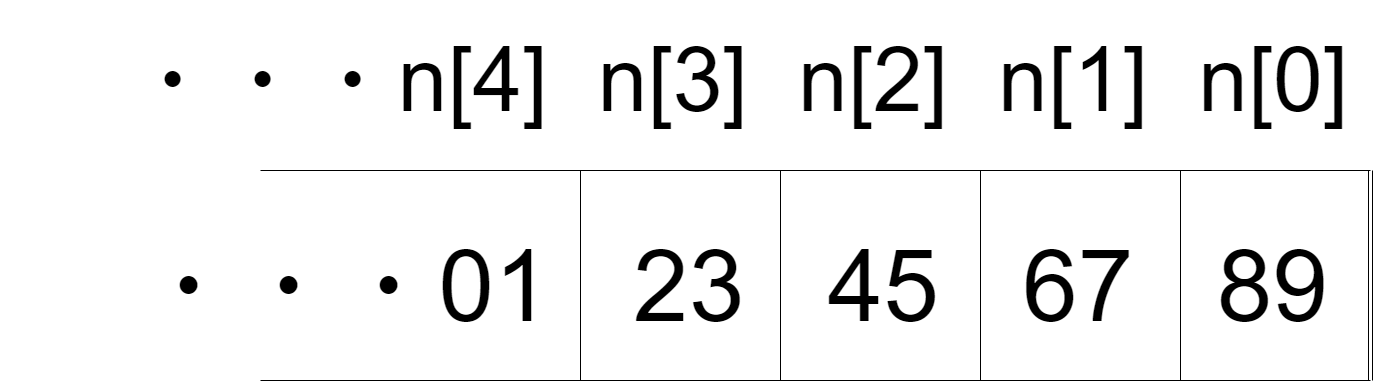
\includegraphics[width=0.5\linewidth]{./images/struct.drawio.png}
  \caption{多倍長整数の構造}
  \label{fig:struct}
\end{figure}

変数\textit{sign}は多倍長整数の符号を表す.
定義の\texttt{PLUS}.\texttt{ZERO},\texttt{MINUS}はそれぞれ正,0,負を表しており,\textit{sign}にはこれらのいずれかが格納される.

多倍長整数の実装を\texttt{pi.h}から抜粋してリスト\ref{lst:pi}に示す.
\begin{lstlisting}[caption=多倍長整数の実装,label=lst:pi]
  typedef struct NUMBER {
      RADIX_T n[KETA];  // 各桁の変数
      int sign;         // 符号変数 -1: 負, 0: 0, 1: 正
  } Number;
\end{lstlisting}

\subsection{関数}
本課題で実装した関数を表\ref{table:function}に示す.
これらの関数について各項で説明する.
\begin{table}[H]
\centering
\caption{関数一覧}
\label{table:function}
\begin{tabular}{c|c}
\hline
関数名    & 機能   \\
\hline
\hline
\textit{setSign}    & 符号を設定する   \\
\hline
\textit{getSign}    & 符号を取得する   \\
\hline
\textit{clearByZero}    & 多倍長整数を初期化する   \\
\hline
\textit{dispNumber}   & 多倍長整数を表示する   \\
\hline
\textit{copyNumber}    & 値をコピーする   \\
\hline
\textit{getAbs}    & 絶対値を求める   \\
\hline
\textit{isZero}    & 0かどうかを判定する   \\
\hline
\textit{mulBy10SomeTimes}    & 何回か10倍する   \\
\hline
\textit{divBy10SomeTimes}    & 何回か10で割る   \\
\hline
\textit{setInt}    & int型の値を多倍長整数に代入する   \\
\hline
\textit{getInt}    & 多倍長整数をint型に変換する   \\
\hline
\textit{numComp}    & 2つの多倍長整数を比較する   \\
\hline
\textit{numCompWithInt}    & 多倍長整数とint型の値を比較する   \\
\hline
\textit{add}    & 2つの多倍長整数を加算する   \\
\hline
\textit{sub}    & 2つの多倍長整数を減算する   \\
\hline
\textit{multiple}    & 2つの多倍長整数を乗算する   \\
\hline
\textit{inverse3}    & 多倍長整数の逆数を求める   \\
\hline
\textit{divideByInverse}   & 2つの多倍長整数を除算する   \\
\hline
\textit{sqrtThree}    & $\sqrt{3}$を求める   \\
\hline
\textit{getLen}    & 多倍長整数の桁数を取得する   \\
\hline
\textit{comparePi}    & 多倍長整数が円周率と等しいかどうか比較する   \\
\hline
\textit{compareRootThree}    & 多倍長整数が$\sqrt{3}$と等しいかどうか比較する   \\
\hline
\end{tabular}
\end{table}

\subsubsection{setSign関数}
\texttt{setSign}関数は表\ref{table:lst:setSign}のように宣言されている.

\begin{table}[H]
\centering
\caption{\texttt{setSign}関数}
\label{table:lst:setSign}
\begin{tabular}{c||c}
\hline
関数名    & \texttt{setSign}   \\
\hline
概要    & 符号を設定する   \\
\hline
引数1    & \texttt{Number *a}: 符号を設定する多倍長整数     \\
引数2    & \texttt{int s}: 設定する符号   \\
\hline
戻り値    & \texttt{int}: 成功した場合は\texttt{TRUE},失敗した場合は\texttt{FALSE}   \\
\hline
\end{tabular}
\end{table}

\texttt{setSign}関数は引数\texttt{s}の値を多倍長整数\texttt{a}の符号に設定する関数である.
それを次の手順でプログラム上で実装する.
\begin{enumerate}
  \item 引数\textit{s}が\textit{PLUS},\textit{ZERO},\textit{MINUS}のいずれかの場合,それぞれ引数\textit{a}の符号を\textit{PLUS},\textit{ZERO},\textit{MINUS}に設定し,\textit{TRUE}を返す.
  \item 引数\textit{s}が\textit{PLUS},\textit{ZERO},\textit{MINUS}のいずれでもない場合,\textit{FALSE}を返す.
\end{enumerate}

\texttt{setSign}関数のソースコードをリスト\ref{lst:setSignsrc}に示す.
\begin{lstlisting}[caption=\texttt{setSign関数},label=lst:setSignsrc]
  int setSign(Number *a, int s) {
    switch (s) {
        case PLUS:
            a->sign = PLUS;
            break;
        case ZERO:
            a->sign = ZERO;
            break;
        case MINUS:
            a->sign = MINUS;
            break;
        default:
            return FALSE;
    }
    return TRUE;
}
\end{lstlisting}

\subsubsection{getSign}
\texttt{getSign}関数は表\ref{table:lst:getSign}のように宣言されている.

\begin{table}[H]
\centering
\caption{\texttt{getSign}関数}
\label{table:lst:getSign}
\begin{tabular}{c||c}
\hline
関数名    & \texttt{getSign}   \\
\hline
概要    & 符号を取得する   \\
\hline
引数    & \texttt{const Number *a}: 符号を取得する多倍長整数   \\
\hline
戻り値    & \texttt{int}: 符号   \\
\hline
\end{tabular}
\end{table}

\textit{const}とは,引数の値を変更しないことを明示するための修飾子である.
関数内で上書き処理を行わない関数では引数に\textit{const}をつけることで,引数の値を変更しないことを明示する.
これはプログラムの保守性を高めるための記述方法であり,以降の関数にも同様の記述がある.

\texttt{getSign}関数は次の手順でプログラム上で多倍長整数の符号を戻り値として返すように実装する.

\texttt{getSign}関数のソースコードをリスト\ref{lst:getSignsrc}に示す.
\begin{lstlisting}[caption=\texttt{getSign}関数,label=lst:getSignsrc]
  int getSign(const Number *a) { return a->sign; }
\end{lstlisting}



\subsubsection{clearByZero}
\texttt{clearByZero}関数は表\ref{table:lst:clearByZero}のように宣言されている.

\begin{table}[H]
\centering
\caption{\texttt{clearByZero}関数}
\label{table:lst:clearByZero}
\begin{tabular}{c||c}
\hline
関数名    & \texttt{clearByZero}   \\
\hline
概要    & 多倍長整数を初期化する   \\
\hline
引数    & \texttt{Number *a}: 初期化する多倍長整数   \\
\hline
戻り値    & なし   \\
\hline
\end{tabular}
\end{table}

リスト\ref{doClearByZero}のように\texttt{clearByZero}関数を呼び出すと,リスト\ref{lst:clearByZero}のように動作する.
\texttt{RADIX}は100,\texttt{RADIX\_LEN}は2とする.また,以降も関数の動作を説明する際にはこの値を用いる.
\begin{lstlisting}[caption=\texttt{clearByZero}関数の呼び出し,label=doClearByZero]
  #include <stdio.h>
  #include "pi.c"
  int main (void){
      Number a;
      clearByZero(&a);
      printf("a: %d\n", a.n[0]);
      printf("sign: %d\n", getSign(&a));
      return 0;
  }
\end{lstlisting}

\begin{lstlisting}[caption=リスト\ref{doClearByZero}の実行結果,label=lst:clearByZero]
  a: 0
  sign: 0
\end{lstlisting}

値が0で初期化され,符号も0に設定されていることがわかる.

\texttt{clearByZero}関数はfor文のループを使って多倍長整数を初期化するように実装する.
\textit{clearByZero}関数のソースコードをリスト\ref{lst:clearByZerosrc}に示す.
\begin{lstlisting}[caption=clearByZero関数,label=lst:clearByZerosrc]
  void clearByZero(Number *a) {
      for (int i = 0; i < KETA; i++) {
          a->n[i] = 0;
      }
      setSign(a, ZERO);
  }
\end{lstlisting}

\subsubsection{dispNumber}
\texttt{dispNumber}関数は表\ref{table:lst:dispNumber}のように宣言されている.

\begin{table}[H]
\centering
\caption{\texttt{dispNumber}関数}
\label{table:lst:dispNumber}
\begin{tabular}{c||c}
\hline
関数名    & \texttt{dispNumber}   \\
\hline
概要    & 多倍長整数を表示する   \\
\hline
引数    & \texttt{const Number *a}: 表示する多倍長整数   \\
\hline
戻り値    & なし   \\
\hline
\end{tabular}

\end{table}

リスト\ref{doDispNumber}のように\texttt{dispNumber}関数を呼び出すと,リスト\ref{lst:dispNumber}のように動作する.
\begin{lstlisting}[caption=\texttt{dispNumber}関数の呼び出し,label=doDispNumber]
  #include "pi.c"
  int main (void){
      Number a;
      clearByZero(&a);
      dispNumber(&a);
      a.n[0] = 12;
      a.n[2] = 34;
      dispNumber(&a);
      printf("\n");
      setSign(&a, MINUS);
      dispNumber(&a);
      printf("\n");
      return 0;
  }
\end{lstlisting}

\begin{lstlisting}[caption=リスト\ref{doDispNumber}の実行結果,label=lst:dispNumber]
  + 0
  + 34 00 12
  - 34 00 12
\end{lstlisting}

リスト\ref{lst:dispNumber}から,\texttt{dispNumber}関数は+,0,-を表示し,その後ろに多倍長整数の各要素を1要素ずつ
表示することがわかる.

次の手順で\texttt{dispNumber}関数を実装する.
\begin{enumerate}
  \item 多倍長整数の符号を判定し,正ならば$+$,0ならば$+$0,負ならば$-$を表示する.
  \item $a_i(i = \texttt{KETA}-1,\texttt{KETA}-2...)$で0でない要素を見つけるまでiを減らす.
  \item $a_i$を表示し,iを減らす.
  \item iが0になるまで3を繰り返す.
\end{enumerate}

この手順をプログラム上では次の手順で実装する.
\begin{enumerate}
  \item 引数aの符号を判定し,正ならば$+$,0ならば$+$0,負ならば$-$を表示する.
  \item 0を付けて表示する書式を設定する.
  \item for文を用いて$i=\texttt{KETA}-1$から,\texttt{a->n[i]}が0ではない要素を見つけるまでiを減らす
  \item for文を用いてiから0まで\texttt{a->n[i]}を表示する.
\end{enumerate}

\texttt{dispNumber}関数のソースコードをリスト\ref{lst:dispNumbersrc}に示す.

\begin{lstlisting}[caption=\texttt{dispNumber}関数,label=lst:dispNumbersrc]
  void dispNumber(const Number *a) {
      int i;
      char format[8];
      sprintf(format, " %%0%dd", RADIX_LEN);  // format = " %0RADIX_LENd"
      switch (getSign(a)) {
          case PLUS:
              printf("+");
              break;
          case ZERO:
              printf("+ 0");
              return;
          case MINUS:
              printf("-");
              break;
      }
      for (i = KETA - 1; i >= 0; i--) {
          if (a->n[i] > 0) {
              break;
          }
      }
      for (; i >= 0; i--) {
          printf(format, a->n[i]);
      }
  }
\end{lstlisting}

\subsubsection{copyNumber}
\texttt{copyNumber}関数は表\ref{table:lst:copyNumber}のように宣言されている.

\begin{table}[H]
\centering
\caption{\texttt{copyNumber}関数}
\label{table:lst:copyNumber}
\begin{tabular}{c||c}
\hline
関数名    & copyNumber   \\
\hline
概要    & 値をコピーする   \\
\hline
引数    & \texttt{Number *a}: コピー先, \texttt{const Number *b}: コピー元   \\
\hline
戻り値    & なし   \\
\hline
\end{tabular}
\end{table}

リスト\ref{doCopyNumber}のようにcopyNumber関数を呼び出すと,リスト\ref{lst:copyNumber}のように動作する.
\begin{lstlisting}[caption=copyNumber関数の呼び出し,label=doCopyNumber]
  #include "pi.c"
  int main (void){
      Number a, b;
      clearByZero(&a);
      clearByZero(&b);
      a.n[0] = 12;
      a.n[2] = 34;
      setSign(&a, PLUS);
      copyNumber(&b, &a);
      dispNumber(&a);
      printf("\n");
      dispNumber(&b);
      printf("\n");
      return 0;
  }
\end{lstlisting}

\begin{lstlisting}[caption=リスト\ref{doCopyNumber}の実行結果,label=lst:copyNumber]
  + 34 00 12
  + 34 00 12
\end{lstlisting}

リスト\ref{lst:copyNumber}の実行結果から,\texttt{copyNumber}関数は引数bに引数aの値をコピーすることがわかる.

\texttt{copyNumber}関数は関数内で引数aのアドレスの値を引数bのアドレスにコピーして実装する.
\texttt{copyNumber}関数のソースコードをリスト\ref{lst:copyNumbersrc}に示す.

\begin{lstlisting}[caption=\texttt{copyNumber}関数,label=lst:copyNumbersrc]
  void copyNumber(Number *a, const Number *b) { *a = *b; }
\end{lstlisting}

\subsubsection{getAbs}
\texttt{getAbs}関数は表\ref{table:lst:getAbs}のように宣言されている.

\begin{table}[H]
\centering
\caption{\texttt{getAbs}関数}
\label{table:lst:getAbs}
\begin{tabular}{c||c}
\hline
関数名    & getAbs   \\
\hline
概要    & 絶対値を求める   \\
\hline
引数    & \texttt{const Number *a}: 絶対値を求める多倍長整数, \texttt{Number *b}: 絶対値を代入する多倍長整数   \\
\hline
戻り値    & なし   \\
\hline
\end{tabular}
\end{table}

リスト\ref{doGetAbs}のように\texttt{getAbs}関数を呼び出すと,リスト\ref{lst:getAbs}のように動作する.
\begin{lstlisting}[caption=\texttt{getAbs}関数の呼び出し,label=doGetAbs]
  #include "pi.c"
  int main (void){
      Number a, b;
      clearByZero(&a);
      clearByZero(&b);
      a.n[0] = 12;
      a.n[2] = 34;
      setSign(&a, MINUS);
      getAbs(&a, &b);
      dispNumber(&a);
      printf("\n");
      dispNumber(&b);
      printf("\n");
      return 0;
  }
\end{lstlisting}

\begin{lstlisting}[caption=リスト\ref{doGetAbs}の実行結果,label=lst:getAbs]
  - 34 00 12
  + 34 00 12
\end{lstlisting}

リスト\ref{lst:getAbs}の実行結果から,\texttt{getAbs}関数は引数aの絶対値を引数bに代入することがわかる.

\texttt{getAbs}関数は次の手順で実装する.
\begin{enumerate}
  \item 多倍長整数\textit{a}の値を多倍長整数\textit{b}にコピーする.
  \item 多倍長整数\textit{a}の符号が0ならば\textit{b}の符号を0に設定する.
  \item 多倍長整数\textit{a}の符号が0でない場合,\textit{b}の符号を正に設定する.
\end{enumerate}

この手順をプログラム上では次の手順で実装する.
\begin{enumerate}
  \item \texttt{copyNumber}関数を用いて引数\textit{a}を\textit{b}にコピーする.
  \item 引数\textit{a}の符号が\textit{ZERO}ならば引数\textit{b}の符号を\textit{ZERO}に設定する.
  \item 引数\textit{a}の符号が\textit{ZERO}でない場合,引数\textit{b}の符号を正に設定する.
\end{enumerate}

\texttt{getAbs}関数のソースコードをリスト\ref{lst:getAbssrc}に示す.

\begin{lstlisting}[caption=getAbs関数,label=lst:getAbssrc]
  void getAbs(const Number *a, Number *b) {
    copyNumber(b, a);
    if (getSign(a) == ZERO) {
        setSign(b, ZERO);
    } else {
        setSign(b, PLUS);
    }
  }
\end{lstlisting}

\subsubsection{isZero}
\texttt{isZero}関数は表\ref{table:lst:isZero}のように宣言されている.

\begin{table}[H]
\centering
\caption{\texttt{isZero}関数}
\label{table:lst:isZero}
\begin{tabular}{c||c}
\hline
関数名    & \texttt{isZero}   \\
\hline
概要    & 0かどうかを判定する   \\
\hline
引数    & \texttt{const Number *a}: 判定する多倍長整数   \\
\hline
戻り値    & \texttt{int}: 0ならば\texttt{TRUE},0でないならば\texttt{FALSE}   \\
\hline
\end{tabular}
\end{table}

リスト\ref{doIsZero}のように\texttt{isZero}関数を呼び出すと,リスト\ref{lst:isZero}のように動作する.
\begin{lstlisting}[caption=\texttt{isZero}関数の呼び出し,label=doIsZero]
  #include "pi.c"
  int main (void){
      Number a;
      clearByZero(&a);
      a.n[0] = 12;
      a.n[2] = 34;
      setSign(&a, PLUS);
      printf("%d\n", isZero(&a));
      clearByZero(&a);
      printf("%d\n", isZero(&a));
      return 0;
  }
\end{lstlisting}

\begin{lstlisting}[caption=リスト\ref{doIsZero}の実行結果,label=lst:isZero]
  0
  1
\end{lstlisting}

リスト\ref{lst:isZero}の実行結果から,\texttt{isZero}関数は引数aが0でないときはTRUEを,0のときはFALSEを返することがわかる.

isZero関数は次の手順で実装する.
\begin{enumerate}
  \item 多倍長整数の符号が0ならば\textit{TRUE}を返す.
  \item 多倍長整数の符号が0でないならば\textit{FALSE}を返す.
\end{enumerate}

この手順をプログラム上では次の手順で実装する.

\begin{enumerate}
  \item \texttt{getSign}関数を用いて引数\textit{a}の符号を取得する.
  \item 符号が\textit{ZERO}ならば\textit{TRUE}を返す.
  \item 符号が\textit{ZERO}でないならば\textit{FALSE}を返す.
\end{enumerate}

\texttt{isZero}関数のソースコードをリスト\ref{lst:isZerosrc}に示す.

\begin{lstlisting}[caption=\texttt{isZero}関数,label=lst:isZerosrc]
  int isZero(const Number *a) {
    if (getSign(a) == ZERO) {
        return TRUE;
    } else {
        return FALSE;
    }
  }
\end{lstlisting}

\subsubsection{mulBy10SomeTimes}
\texttt{mulBy10SomeTimes}関数は表\ref{table:lst:mulBy10SomeTimes}のように宣言されている.

\begin{table}[H]
\centering
\caption{\texttt{mulBy10SomeTimes}関数}
\label{table:lst:mulBy10SomeTimes}
\begin{tabular}{c||c}
\hline
関数名    & \texttt{mulBy10SomeTimes}   \\
\hline
概要    & 何回か10倍する   \\
\hline
引数1   & \texttt{const Number *a}: 10倍する多倍長整数  \\
引数2   & \texttt{Number *b}: 10倍した結果を代入する多倍長整数  \\
引数3   & \texttt{int k}: 10倍する回数   \\
\hline
戻り値    & \texttt{int}: 成功した場合は\texttt{TRUE},失敗した場合は\texttt{FALSE}   \\
\hline
\end{tabular}
\end{table}

リスト\ref{doMulBy10SomeTimes}のように\texttt{mulBy10SomeTimes}関数を呼び出すと,リスト\ref{lst:mulBy10SomeTimes}のように動作する.
\begin{lstlisting}[caption=\texttt{mulBy10SomeTimes}関数の呼び出し,label=doMulBy10SomeTimes]
  #include "pi.c"
  int main (void){
      Number a, b;
      clearByZero(&a);
      clearByZero(&b)
      a.n[0] = 12;
      a.n[2] = 34;
      setSign(&a, PLUS);
      mulBy10SomeTimes(&a, &b, 2);
      dispNumber(&a);
      printf("\n");
      dispNumber(&b);
      printf("\n");
      return 0;
  }
\end{lstlisting}

\begin{lstlisting}[caption=リスト\ref{doMulBy10SomeTimes}の実行結果,label=lst:mulBy10SomeTimes]
  + 34 00 12
  + 34 00 12 00
\end{lstlisting}

リスト\ref{lst:mulBy10SomeTimes}の実行結果から,\texttt{mulBy10SomeTimes}関数は引数\texttt{a}を引数\texttt{k}回だけ10倍して引数\texttt{b}に代入
することがわかる.

mulBy10SomeTimes関数は次の手順で実装する.
この手順を模式的に示した図を図\ref{fig:mulBy10SomeTimes1}に示す.
\begin{enumerate}
  \item 多倍長整数を$10^k$倍したときの桁数が多倍長整数に格納できる桁数を超える場合,\textit{FALSE}を返す.(図\ref{fig:mulBy10SomeTimes1}の手順1)
  \item 多倍長整数を\textit{k / RADIX\_LEN}要素数,上位要素に移動させる.(図\ref{fig:mulBy10SomeTimes1}の手順2)
  \item 多倍長整数をk \% RADIX\_LEN桁数,上位桁に移動させる.(図\ref{fig:mulBy10SomeTimes1}の手順3)
  \item 移動後の多倍長整数の下位桁を0で埋める.
  \item 符号を設定する.
  \item TRUEを返す.
\end{enumerate}

\begin{figure}[H]
  \centering
  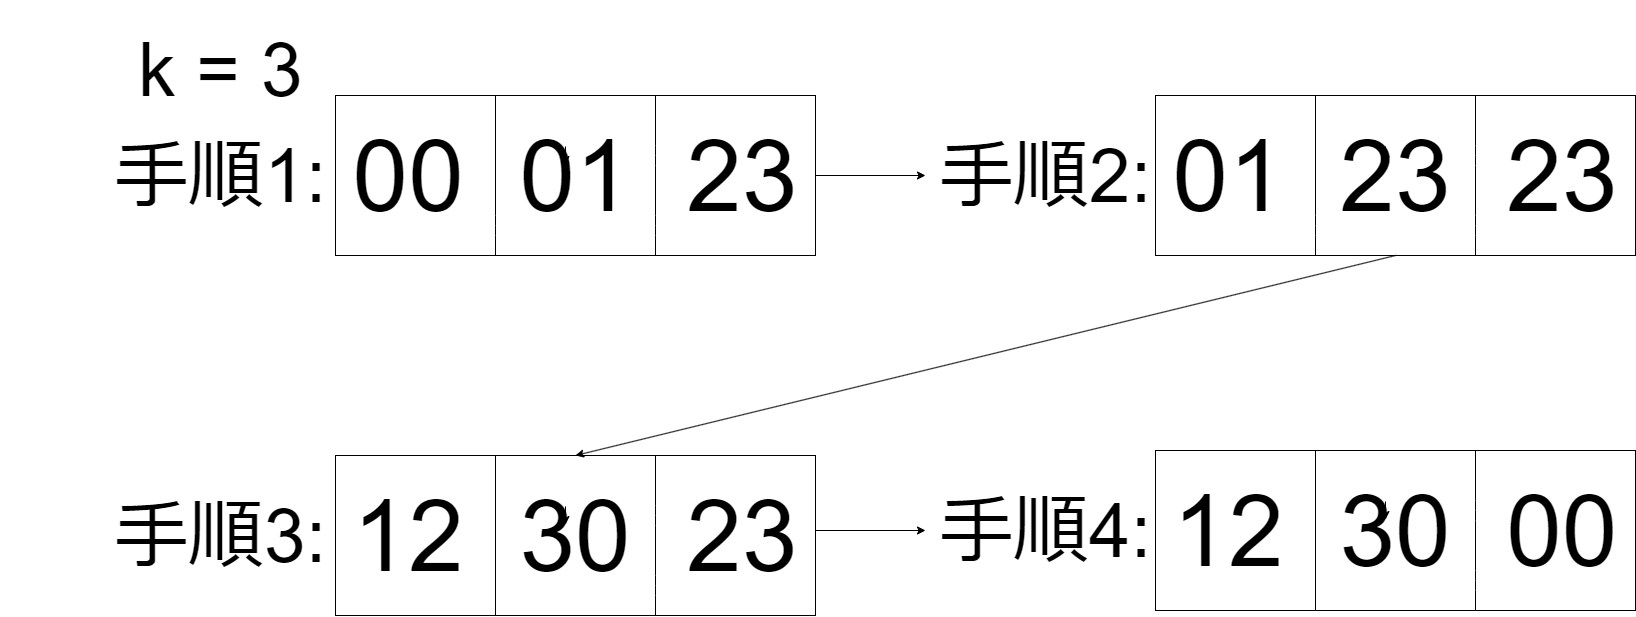
\includegraphics[width=10cm]{./images/mulby10sometimes1.drawio.png}
  \caption{\texttt{mulBy10SomeTimes}関数の手順}
  \label{fig:mulBy10SomeTimes1}
\end{figure}

この手順をプログラム上では次の手順で実装する.
\begin{enumerate}
  \item kがRADIX\_LENよりも大きい場合,k / RADIX\_LEN要素数,上位要素に移動させても多倍長整数に値を格納できるかどうかを判定する.\\
  格納できない場合,FALSEを返す.
  \item 1に加えて,RADIX\_LEN - k \% RADIX\_LEN桁数,上位桁に移動させても多倍長整数に値を格納できるかどうかを判定する.\\
  格納できない場合,FALSEを返す.
  \item 1と2が共に格納できる場合,以下の処理を繰り返す.(前述している手順の手順2にあたる)
  \begin{enumerate}
    \item \textit{a}-\verb|>|\textit{[i + k / RADIX\_LEN](i=多倍長整数の要素数)}に\textit{a}-\verb|>|[i]を代入する.
    \item iを1減らす.
    \item iが0になるまで繰り返す.
  \end{enumerate}
    \item 以下の処理を繰り返す.(前述している手順の手順4にあたる)
    \begin{enumerate}
  \item \textit{a}-\verb|>|[i](i=0)に0を代入する.
  \item \textit{i}を1増やす.
  \item \textit{i}が\textit{k / RADIX\_LEN}になるまで繰り返す.
\end{enumerate}
\item 以下の処理を繰り返す.(前述している手順の手順3にあたる)
  \begin{enumerate}
    \item \textit{a}-\verb|>|[i](i=0)に$10^{k \% RADIX\_LEN}$かける.
    \item 前の桁からの繰り上がり変数\textit{carry}を\textit{a}-\verb|>|[i]に加える.
    \item \textit{a}-\verb|>|[i]がRADIXより大きい場合,\textit{a}-\verb|>|[i] / \textit{RADIX}を\textit{carry}に代入し,
    \textit{a}-\verb|>|[i]に\textit{a}-\verb|>|[i] \% \textit{RADIX}を代入する.
    \item $a_i$がRADIXより小さい場合,carryに0を代入する.
    \item iを1増やす.
    \item iが\textit{aの要素数}になるまで繰り返す.
  \end{enumerate}
  \item 符号を設定する.
  \item TRUEを返す.
\end{enumerate}

10倍する処理を手順3と手順5に分けているのは,一回の処理で要素を$10^k$倍すると,kが大きい場合に数が配列に格納できる最大値を
超え,オーバーフローが発生するためである.

mulBy10SomeTimes関数のソースコードをリスト\ref{lst:mulBy10SomeTimessrc}に示す.

\begin{lstlisting}[caption=mulBy10SomeTimes関数,label=lst:mulBy10SomeTimessrc]
    int mulBy10SomeTimes(const Number *a, Number *b, int k) {
        int rtn = -2;
        int i, j;
        copyNumber(b, a);
        if (isZero(a)) {
            rtn = TRUE;
        } else if (k == 0) {
            rtn = TRUE;
        } else {
            int digit;
            RADIX_T carry;
            digit = k / RADIX_LEN;
            int length = getLen(b);
            j = 0;
            i = KETA - 1;
            while (1) {
                if (digit <= j) {
                    break;
                } else if (b->n[i] != 0) {
                    printf("mulBy10SomeTimes: overflow: -1A\n");
                    rtn = FALSE;
                    break;
                }
                j++;
                i--;
            }
            if (rtn == FALSE) {
                printf("mulBy10SomeTimes: overflow: -1B\n");
            } else if (b->n[i] /
                           (int)pow(10, (RADIX_LEN - (k % RADIX_LEN))) !=
                       0) {
                printf("mulBy10SomeTimes: overflow\n");
                rtn = FALSE;
            } else {
                if (digit != 0) {
                    for (i = length / RADIX_LEN; i >= 0; i--) {
                        b->n[i + digit] = b->n[i];
                    }
                    for (i = 0; i < digit; i++) {
                        b->n[i] = 0;
                    }
                }
                length += digit * RADIX_LEN;
                carry = 0;
                for (i = 0; i < length / RADIX_LEN + 2; i++) {
                    b->n[i] *= (int)pow(10, (k % RADIX_LEN));
                    b->n[i] += carry;
                    if (b->n[i] >= RADIX) {
                        carry = b->n[i] / RADIX;
                        b->n[i] %= RADIX;
                    } else {
                        carry = 0;
                    }
                }
                rtn = TRUE;
            }
        }
        return rtn;
    }
\end{lstlisting}

\subsubsection{divBy10SomeTimes}
\texttt{divBy10SomeTimes}関数は表\ref{table:lst:divBy10SomeTimes}のように宣言されている.

\begin{table}[H]
\centering
\caption{\texttt{divBy10SomeTimes}関数}
\label{table:lst:divBy10SomeTimes}
\begin{tabular}{c||c}
\hline
関数名    & \texttt{divBy10SomeTimes}   \\
\hline
概要    & 何回か10分の1する   \\
\hline
引数1   & \texttt{const Number *a}: 10分の1する多倍長整数  \\
引数2   & \texttt{Number *b}: 10分の1した結果を代入する多倍長整数  \\
引数3   & \texttt{int k}: 10分の1する回数   \\
\hline
戻り値    & なし   \\
\hline
\end{tabular}
\end{table}

リスト\ref{doDivBy10SomeTimes}のように\texttt{divBy10SomeTimes}関数を呼び出すと,リスト\ref{lst:divBy10SomeTimes}のように動作する.
\begin{lstlisting}[caption=\texttt{divBy10SomeTimes}関数の呼び出し,label=doDivBy10SomeTimes]
  #include "pi.c"
  int main (void){
      Number a, b;
      clearByZero(&a);
      clearByZero(&b)
      a.n[0] = 12;
      a.n[2] = 34;
      setSign(&a, PLUS);
      divBy10SomeTimes(&a, &b, 3);
      dispNumber(&a);
      printf("\n");
      dispNumber(&b);
      printf("\n");
      return 0;
  }
\end{lstlisting}

\begin{lstlisting}[caption=リスト\ref{doDivBy10SomeTimes}の実行結果,label=lst:divBy10SomeTimes]
  + 34 00 12
  + 03 40
\end{lstlisting}

リスト\ref{lst:divBy10SomeTimes}の実行結果から,\texttt{divBy10SomeTimes}関数は引数\texttt{a}を引数\texttt{k}回だけ
10分の1して引数\texttt{b}に代入する動作をすることがわかる.

divBy10SomeTimes関数は次の手順で実装する.

\begin{enumerate}
    \item 多倍長整数を\textit{k \% RADIX\_LEN}桁数,下位桁に移動させる.
    \item 多倍長整数を\textit{k / RADIX\_LEN}要素数,下位要素に移動させる.
    \item 移動後の多倍長整数の上位桁を0で埋める.
    \item 符号を設定する.
\end{enumerate}

この手順をプログラム上では次の手順で実装する.

\begin{enumerate}
    \item \textit{b}-\verb|>|[0]を$10^k$で割った値を\textit{b}-\verb|>|[0]に代入する.
    \item 以下の処理を繰り返す(前述する手順の手順1にあたる).
    \begin{enumerate}
    \item \textit{b}-\verb|>|\textit{[i](i=1)}を$10^k$で割った値を\textit{carry}に代入する.
    \item \textit{b}-\verb|>|\textit{[i - 1]}に$carry \times 10^{RADIX\_LEN - (k \% RADIX\_LEN)}$を加える.
    \item \textit{b}-\verb|>|\textit{[i]}から\textit{carry}を引き,$10^{k \% RADIX\_LEN}$で割った値を\textit{b}-\verb|>|\textit{[i]}に代入する.
    \item iを1増やす.
    \item iが\textit{KETA}になるまで繰り返す.
    \end{enumerate}
    \item 以下の処理を繰り返す(前述している手順の手順2にあたる).
    \begin{enumerate}
        \item \textit{b}-\verb|>|\textit{[i](i=0)}に\textit{b}-\verb|>|\textit{[i + k / RADIX\_LEN]}を代入する.
        \item iを1増やす.
        \item iが\textit{KETA - k / RADIX\_LEN}になるまで繰り返す.
    \end{enumerate}
    \item 以下の処理を繰り返す(前述している手順の手順3にあたる).
    \begin{enumerate}
        \item \textit{b}-\verb|>|\textit{[i](i=KETA - k / RADIX\_LEN)}に0を代入する.
        \item iを1増やす.
        \item iが\textit{KETA}になるまで繰り返す.
    \end{enumerate}
\end{enumerate}

divBy10SomeTimes関数のソースコードをリスト\ref{lst:divBy10SomeTimessrc}に示す.

\begin{lstlisting}[caption=divBy10SomeTimes関数,label=lst:divBy10SomeTimessrc]
    void divBy10SomeTimes(const Number *a, Number *b, int k) {
        int i;
        int digit;
        int carry;
        digit = k / RADIX_LEN;
        copyNumber(b, a);
        b->n[0] -= b->n[0] % (int)pow(10, k % RADIX_LEN);
        b->n[0] /= (int)pow(10, k % RADIX_LEN);
        for (i = 1; i < KETA; i++) {
            carry = b->n[i] % (int)pow(10, k % RADIX_LEN);
            b->n[i - 1] +=
                carry * (int)pow(10, RADIX_LEN - (k % RADIX_LEN));
            b->n[i] -= carry;
            b->n[i] /= (int)pow(10, k % RADIX_LEN);
        }
        if (digit > 0) {
            for (i = 0; i < KETA - digit; i++) {
                b->n[i] = b->n[i + digit];
            }
            for (i = KETA - digit; i < KETA; i++) {
                b->n[i] = 0;
            }
        }
        return;
    }
\end{lstlisting}

\subsubsection{setInt}
\texttt{setInt}関数は表\ref{table:lst:setInt}のように宣言されている.

\begin{table}[H]
\centering
\caption{\texttt{setInt}関数}
\label{table:lst:setInt}
\begin{tabular}{c||c}
\hline
関数名    & \texttt{setInt}   \\
\hline
概要    & 整数を多倍長整数に設定する   \\
\hline
引数1   & \texttt{Number *a}: 設定する多倍長整数  \\
引数2   & \texttt{long n}: 設定する整数  \\
\hline
戻り値    & \texttt{int}: 成功した場合は\texttt{TRUE},失敗した場合は\texttt{FALSE}   \\
\hline
\end{tabular}
\end{table}

リスト\ref{doSetInt}のように\texttt{setInt}関数を呼び出すと,リスト\ref{lst:setInt}のように動作する.
\begin{lstlisting}[caption=\texttt{setInt}関数の呼び出し,label=doSetInt]
    #include "pi.c"
    int main (void){
        Number a;
        setInt(&a, 1234);
        dispNumber(&a);
        printf("\n");
        return 0;
    }
\end{lstlisting}

\begin{lstlisting}[caption=リスト\ref{doSetInt}の実行結果,label=lst:setInt]
    + 12 34
\end{lstlisting}

リスト\ref{lst:setInt}の実行結果から,\texttt{setInt}関数は引数\texttt{n}を引数\texttt{a}に代入するという動作をすることがわかる.

setInt関数は次の手順で実装する.
\begin{enumerate}
    \item 引数\textit{n}が0の場合,多倍長整数\textit{a}の符号を\textit{ZERO}に設定する.
    \item 引数\textit{n}が負の値の場合,多倍長整数\textit{a}の符号を\textit{MINUS}に設定し,引数\textit{n}をプラスに変換する.
    \item 引数\textit{n}が正の値の場合,多倍長整数\textit{a}の符号を\textit{PLUS}に設定する.
    \item 引数\textit{n}を多倍長整数\textit{a}に代入する.
    \item TRUEを返す.
\end{enumerate}

この手順をプログラム上では次の手順で実装する.
\begin{enumerate}
    \item 引数\textit{n}が負の値の場合,\textit{setSign}関数で引数\textit{a}の符号を\textit{MINUS}に設定し,
    \textit{n}をプラスに変換する.
    \item 引数\textit{n}が0の場合,\textit{setSign}関数で引数\textit{a}の符号を\textit{ZERO}に設定する.
    \item 引数\textit{n}が正の値の場合,\textit{setSign}関数で引数\textit{a}の符号を\textit{PLUS}に設定する.
    \item 引数\textit{n}の先頭の配列要素に\textit{n}を代入する.
    \item TRUEを返す.
\end{enumerate}

この関数では,引数\textit{n}が多倍長整数の基数を超える場合には対応していない.
そのため,引数\textit{n}が多倍長整数の基数を超える場合には,正しく動作しない点に注意が必要である.
setInt関数のソースコードをリスト\ref{lst:setIntsrc}に示す.

\begin{lstlisting}[caption=setInt関数,label=lst:setIntsrc]
    int setInt(Number *a, long x) {
        clearByZero(a);
        if (x < 0) {
            setSign(a, MINUS);
            x *= -1;
        } else if (x == 0) {
            setSign(a, ZERO);
        } else {
            setSign(a, PLUS);
        }
        a->n[0] = x % RADIX;
        return TRUE;
    }
\end{lstlisting}

\subsubsection{getInt}
\texttt{getInt}関数は表\ref{table:lst:getInt}のように宣言されている.

\begin{table}[H]
\centering
\caption{\texttt{getInt}関数}
\label{table:lst:getInt}
\begin{tabular}{c||c}
\hline
関数名    & \texttt{getInt}   \\
\hline
概要    & 多倍長整数を整数に変換する   \\
\hline
引数1   & \texttt{const Number *a}: 変換する多倍長整数  \\
引数2   & \texttt{int *x}: 変換した整数を代入する変数  \\
\hline
戻り値    & \texttt{int}: 成功した場合は\texttt{TRUE},失敗した場合は\texttt{FALSE}   \\
\hline
\end{tabular}
\end{table}

リスト\ref{doGetInt}のように\texttt{getInt}関数を呼び出すと,リスト\ref{lst:getInt}のように動作する.
\begin{lstlisting}[caption=\texttt{getInt}関数の呼び出し,label=doGetInt]
    #include "pi.c"
    int main (void){
        Number a;
        int x;
        setInt(&a, 1234);
        dispNumber(&a);
        printf("\n");
        getInt(&a, &x);
        printf("%d\n", x);
        return 0;
    }
\end{lstlisting}

\begin{lstlisting}[caption=リスト\ref{doGetInt}の実行結果,label=lst:getInt]
    + 12 34
    1234
\end{lstlisting}

リスト\ref{lst:getInt}の実行結果から,\texttt{getInt}関数は引数\texttt{a}を整数に変換して引数\texttt{x}に代入するという
動作をすることがわかる.

getInt関数は次の手順で実装する.
\begin{enumerate}
    \item 多倍長整数\textit{a}の符号が\textit{ZERO}の場合,0を返す.
    \item 多倍長整数の値を変数\textit{x}に代入する.
    \item 多倍長整数の符号が\textit{MINUS}の場合,\textit{x}に-1を掛ける.
    \item TRUEを返す.
\end{enumerate}

この手順をプログラム上では次の手順で実装する.
\begin{enumerate}
    \item 引数\textit{a}が0の場合,引数\textit{x}に0を代入し,\textit{TRUE}を返す.
    \item 引数\textit{a}の桁数がRADIX\_LENよりも大きい場合,\textit{FALSE}を返す.
    \item 引数\textit{a}の先頭の配列要素を\textit{x}に代入する.
    \item 引数\textit{a}の符号を\textit{getSign}で取得し,それが\textit{MINUS}の場合,\textit{x}に-1を掛ける.
    \item TRUEを返す.
\end{enumerate}

この関数では,多倍長整数の値がint型の範囲を超える場合には対応していない.
そのため,多倍長整数の値がint型の範囲を超える場合には,正しく動作しない点に注意が必要である.

getInt関数のソースコードをリスト\ref{lst:getIntsrc}に示す.

\begin{lstlisting}[caption=getInt関数,label=lst:getIntsrc]
    int getInt(const Number *a, int *x) {
        int rtn;
        if (isZero(a)) {
            *x = 0;
            rtn = TRUE;
        } else if (getLen(a) > RADIX_LEN) {
            rtn = FALSE;
        } else {
            *x = a->n[0];
            *x += a->n[1] * RADIX;
            if (getSign(a) == MINUS) {
                *x *= -1;
            }
            rtn = TRUE;
        }
        return rtn;
    }
\end{lstlisting}

\subsubsection{numComp}
\texttt{numComp}関数は表\ref{table:lst:numComp}のように宣言されている.

\begin{table}[H]
\centering
\caption{\texttt{numComp}関数}
\label{table:lst:numComp}
\begin{tabular}{c||c}
\hline
関数名    & \texttt{numComp}   \\
\hline
概要    & 2つの多倍長整数を比較する   \\
\hline
引数1   & \texttt{const Number *a}: 比較する多倍長整数1  \\
引数2   & \texttt{const Number *b}: 比較する多倍長整数2  \\
\hline
戻り値    & \texttt{int}: \texttt{a}が\texttt{b}より大きい場合は1,\texttt{a}が\texttt{b}より小さい場合は-1,等しい場合は0を返す   \\
\hline
\end{tabular}
\end{table}

リスト\ref{doNumComp}のように\texttt{numComp}関数を呼び出すと,リスト\ref{lst:numComp}のように動作する.
\begin{lstlisting}[caption=\texttt{numComp}関数の呼び出し,label=doNumComp]
    #include "pi.c"
    int main (void){
        Number a, b;
        int rtn;
        setInt(&a, 1234);
        setInt(&b, 1234);
        rtn = numComp(&a, &b);
        dispNumber(&a);
        printf("\n");
        dispNumber(&b);
        printf("\n");
        printf("%d\n", rtn);
        setInt(&b, 1235);
        rtn = numComp(&a, &b);
        dispNumber(&a);
        printf("\n");
        dispNumber(&b);
        printf("\n");
        printf("%d\n", rtn);
        setInt(&b, 1233);
        rtn = numComp(&a, &b);
        dispNumber(&a);
        printf("\n");
        dispNumber(&b);
        printf("\n");
        printf("%d\n", rtn);
        return 0;
    }
\end{lstlisting}

\begin{lstlisting}[caption=リスト\ref{doNumComp}の実行結果,label=lst:numComp]
    + 12 34
    + 12 34
    0
    + 12 34
    + 12 35
    -1
    + 12 34
    + 12 33
    1
\end{lstlisting}

リスト\ref{lst:numComp}の実行結果から,\texttt{numComp}関数は引数\texttt{a}と引数\texttt{b}を比較して,\texttt{a}が\texttt{b}より大きい場合は1,
\texttt{a}が\texttt{b}より小さい場合は-1,等しい場合は0を返すという動作をすることがわかる.

numComp関数は次の手順で実装する.
\begin{enumerate}
    \item 多倍長整数\textit{a}と多倍長整数\textit{b}の符号が異なる場合は符号での比較を行い,比較結果に応じて1または-1を返す.
    \item 多倍長整数\textit{a}と多倍長整数\textit{b}の符号が同じ場合は,多倍長整数\textit{a}と多倍長整数\textit{b}の絶対値を比較し,
    符号に応じて結果を返す.
\end{enumerate}

この手順をプログラム上では次の手順で実装する.
\begin{enumerate}
    \item 引数\textit{a}と引数\textit{b}の符号によって場合わけをし,以下の処理を行う.
    \begin{itemize}
        \item 引数\textit{a}の符号が\textit{MINUS}で引数\textit{b}の符号が\textit{PLUS}の場合,-1を返す.
        \item 引数\textit{a}の符号が\textit{PLUS}で引数\textit{b}の符号が\textit{MINUS}の場合,1を返す.
        \item 引数\textit{a}の符号が\textit{ZERO}で引数\textit{b}の符号が\textit{ZERO}の場合,0を返す.
        \item 引数\textit{a}の符号が\textit{PLUS}で引数\textit{b}の符号が\textit{ZERO}の場合,1を返す.
        \item 引数\textit{a}の符号が\textit{MINUS}で引数\textit{b}の符号が\textit{ZERO}の場合,-1を返す.
        \item 引数\textit{a}の符号が\textit{ZERO}で引数\textit{b}の符号が\textit{PLUS}の場合,-1を返す.
        \item 引数\textit{a}の符号が\textit{ZERO}で引数\textit{b}の符号が\textit{MINUS}の場合,1を返す.
        \item 引数\textit{a}の符号が\textit{PLUS}で引数\textit{b}の符号が\textit{PLUS}の場合や,引数\textit{a}の符号が\textit{MINUS}で引数\textit{b}の符号が\textit{MINUS}の場合,手順2に進む.
    \end{itemize}
    \item 桁数を比較し,結果に応じて1または-1を返す.
    \item 桁数が同じな場合,上位の桁から比較し,結果に応じて1または-1を返す.
    \item すべての桁が同じ場合,0を返す.
\end{enumerate}

numComp関数のソースコードをリスト\ref{lst:numCompsrc}に示す.

\begin{lstlisting}[caption=\texttt{numComp}関数,label=lst:numCompsrc]
    int numComp(const Number *a, const Number *b) {
        int rtn = 0;
        switch (getSign(a) * 3 + getSign(b)) {
            case -4:  // aとbが負
                if (getLen(a) > getLen(b)) {
                    rtn = -1;
                } else if (getLen(a) < getLen(b)) {
                    rtn = 1;
                }
                for (int i = KETA - 1; i >= 0; i--) {
                    if (a->n[i] < b->n[i]) {
                        rtn = 1;
                        break;
                    } else if (a->n[i] > b->n[i]) {
                        rtn = -1;
                        break;
                    }
                }
                break;
            case 4:  // aとbが正
                if (getLen(a) > getLen(b)) {
                    rtn = 1;
                } else if (getLen(a) < getLen(b)) {
                    rtn = -1;
                }
                for (int i = KETA - 1; i >= 0; i--) {
                    if (a->n[i] > b->n[i]) {
                        rtn = 1;
                        break;
                    } else if (a->n[i] < b->n[i]) {
                        rtn = -1;
                        break;
                    }
                }
                break;
            case -3:  // aが負でbが0
            case -2:  // aが負でbが正
            case 1:   // aが0でbが正
                rtn = -1;
                break;
            case -1:  // aが0でbが負
            case 2:   // aが正でbが負
            case 3:   // aが正でbが0
                rtn = 1;
                break;
            case 0:  // aとbが0
                break;
        }
        return rtn;
    }
\end{lstlisting}

\subsubsection{numCompWithInt}
\texttt{numCompWithInt}関数は表\ref{table:lst:numCompWithInt}のように宣言されている.

\begin{table}[H]
\centering
\caption{\texttt{numCompWithInt}関数}
\label{table:lst:numCompWithInt}
\begin{tabular}{c||c}
\hline
関数名    & \texttt{numCompWithInt}   \\
\hline
概要    & 多倍長整数とint型整数を比較する   \\
\hline
引数1   & \texttt{const Number *a}: 比較する多倍長整数  \\
引数2   & \texttt{int b}: 比較するint型整数  \\
\hline
戻り値    & \texttt{int}: \texttt{a}が\texttt{b}より大きい場合は1,\texttt{a}が\texttt{b}より小さい場合は-1,等しい場合は0を返す   \\
\hline
\end{tabular}
\end{table}

リスト\ref{doNumCompWithInt}のように\texttt{numCompWithInt}関数を呼び出すと,リスト\ref{lst:numCompWithInt}のように動作する.

\begin{lstlisting}[caption=\texttt{numCompWithInt}関数の呼び出し,label=doNumCompWithInt]
    #include "pi.c"
    int main (void){
        Number a;
        int rtn;
        setInt(&a, 1234);
        rtn = numCompWithInt(&a, 1234);
        dispNumber(&a);
        printf("\n");
        printf("%d\n", rtn);
        rtn = numCompWithInt(&a, 1235);
        dispNumber(&a);
        printf("\n");
        printf("%d\n", rtn);
        rtn = numCompWithInt(&a, 1233);
        dispNumber(&a);
        printf("\n");
        printf("%d\n", rtn);
        return 0;
    }
\end{lstlisting}

\begin{lstlisting}[caption=リスト\ref{doNumCompWithInt}の実行結果,label=lst:numCompWithInt]
    + 12 34
    0
    + 12 34
    -1
    + 12 34
    1
\end{lstlisting}

リスト\ref{lst:numCompWithInt}の実行結果から,\texttt{numCompWithInt}関数は引数\texttt{a}と引数\texttt{b}を比較して,
\texttt{a}が\texttt{b}より大きい場合は1,\texttt{a}が\texttt{b}より小さい場合は-1,等しい場合は0を返すという動作をすることがわかる.

numCompWithInt関数は多倍長整数\textit{a}をint型整数に変換し,引数\textit{x}と比較して,比較結果に応じて戻り値を返すことで動作する.

その動作をプログラム上で次の手順で実装する.
\begin{enumerate}
    \item 引数\textit{a}を\textit{getInt}関数でint型整数に変換する.
    \item 変換に失敗した場合,1を返す.
    \item int型に変換した整数と引数\textit{b}を比較し,比較結果に応じて戻り値を返す.
\end{enumerate}

numCompWithInt関数のソースコードをリスト\ref{lst:numCompWithIntsrc}に示す.

\begin{lstlisting}[caption=\texttt{numCompWithInt}関数,label=lst:numCompWithIntsrc]
    int numCompWithInt(const Number *a, int x) {
        int num, rtn;
        if (getInt(a, &num) == FALSE) {
            rtn = TRUE;
        } else if (num > x) {
            rtn = TRUE;
        } else if (num < x) {
            rtn = FALSE;
        } else {
            rtn = 0;
        }
        return rtn;
    }
\end{lstlisting}

\subsubsection{add, sub}
\texttt{add}関数と\texttt{sub}関数は表\ref{table:lst:add},表\ref{table:lst:sub}のように宣言されている.

\begin{table}[H]
\centering
\caption{\texttt{add}関数}
\label{table:lst:add}
\begin{tabular}{c||c}
\hline
関数名    & \texttt{add}   \\
\hline
概要    & 2つの多倍長整数を加算する   \\
\hline
引数1   & \texttt{const Number *a}: 加算する多倍長整数1  \\
引数2   & \texttt{const Number *b}: 加算する多倍長整数2  \\
引数3   & \texttt{Number *c}: 加算結果を代入する多倍長整数  \\
\hline
戻り値    & \texttt{int}: 成功した場合は\texttt{TRUE},失敗した場合は\texttt{FALSE}   \\
\hline
\end{tabular}
\end{table}

\begin{table}[H]
\centering
\caption{\texttt{sub}関数}
\label{table:lst:sub}
\begin{tabular}{c||c}
\hline
関数名    & \texttt{sub}   \\
\hline
概要    & 2つの多倍長整数を減算する   \\
\hline
引数1   & \texttt{const Number *a}: 減算する多倍長整数1  \\
引数2   & \texttt{const Number *b}: 減算する多倍長整数2  \\
引数3   & \texttt{Number *c}: 減算結果を代入する多倍長整数  \\
\hline
戻り値    & \texttt{int}: 成功した場合は\texttt{TRUE},失敗した場合は\texttt{FALSE}   \\
\hline
\end{tabular}
\end{table}

リスト\ref{doAddSub}のように\texttt{add}関数と\texttt{sub}関数を呼び出すと,リスト\ref{lst:addsub}のように動作する.

\begin{lstlisting}[caption=\texttt{add}関数と\texttt{sub}関数の呼び出し,label=doAddSub]
    #include "pi.c"
    int main (void){
        Number a, b, c;
        int rtn;
        setInt(&a, 1234);
        setInt(&b, 5678);
        rtn = add(&a, &b, &c);
        dispNumber(&a);
        printf(" + ");
        dispNumber(&b);
        printf(" = ");
        dispNumber(&c);
        printf("\n");
        printf("%d\n", rtn);
        rtn = sub(&a, &b, &c);
        dispNumber(&a);
        printf(" - ");
        dispNumber(&b);
        printf(" = ");
        dispNumber(&c);
        printf("\n");
        printf("%d\n", rtn);
        return 0;
    }
\end{lstlisting}
\begin{lstlisting}[caption=リスト\ref{doAddSub}の実行結果,label=lst:addsub]
    + 12 34 + + 56 78 = 69 12
    1
    + 12 34 - + 56 78 = - 44 44
    
\end{lstlisting}

リスト\ref{lst:addsub}の実行結果から,\texttt{add}関数と\texttt{sub}関数は引数\texttt{a}と引数\texttt{b}を加算,減算して,
引数\texttt{c}に代入するという動作をすることがわかる.

add関数とsub関数はどちらも符号で場合分けをし,式を変形してから計算を行っている.
add関数の式変形は次のように行っている.
\begin{itemize}
    \item aが正,bが正の場合,$a + b = a + b$
    \item aが正,bが負の場合,$a + b = a - |b|$
    \item aが負,bが正の場合,$a + b = b - |a|$
    \item aが負,bが負の場合,$(-a) + (-b) = -(|a| + |b|)$
    \item aが0の場合,$a + b = b$
    \item bが0の場合,$a + b = a$
\end{itemize}

sub関数の式変形は次のように行っている.
\begin{itemize}
    \item aが正,bが正の場合,$a - b = a - b$
    \item aが正,bが負の場合,$a - b = a + |b|$
    \item aが負,bが正の場合,$a - b = -(|a| + b)$
    \item aが負,bが負の場合,$a - b = |a| - |b|$
    \item aが0の場合,$a - b = -b$
    \item bが0の場合,$a - b = a$
\end{itemize}

なので,add関数とsub関数ともに,引数\texttt{a}と引数\texttt{b}の符号がどちらも正の場合の計算手順を示す.
add関数の計算手順は次のようになる.

\begin{enumerate}
        \item 多倍長整数$a_i(i = 0)$と多倍長整数$b_i$と\textit{carry}を加算し,変数\textit{num}に代入する
        \item 変数\textit{num}が\textit{RADIX}より大きい場合,変数\textit{num}を\textit{RADIX}で割った余りを多倍長整数$c_i$に代入し,
        繰り上がりとして変数\textit{carry}に1を代入する.
        \item 変数\textit{num}が\textit{RADIX}以下の場合,変数\textit{num}を多倍長整数$c_i$に代入し,繰り上がりなしとして変数\textit{carry}に0を代入する.
        \item \textit{i}を1増やす.
        \item \textit{i}が多倍長整数の要素数に達するまで手順1から4を繰り返す.
        \item ループを抜けた後,繰り上がりがある場合,多倍長整数に格納できないのでオーバーフローとして\textit{FALSE}を返す.
        \item 繰り上がりがない場合,\textit{TRUE}を返す.
\end{enumerate}

sub関数の計算手順は次のようになる.

\begin{enumerate}
        \item 多倍長整数$a_i(i = 0)$かr繰り下がり変数\textit{carry}を減算し,変数\textit{num}に代入する
        \item 変数\textit{num}が$b_i$より小さい場合,変数\textit{num}に\textit{RADIX}を加え,繰り下がりとして変数\textit{carry}に1を代入する.
        \item 変数\textit{num}が$b_i$以上の場合,変数\textit{num}を多倍長整数$c_i$に代入し,繰り下がりなしとして変数\textit{carry}に0を代入する.
        \item \textit{i}を1増やす.
        \item \textit{i}が多倍長整数の要素数に達するまで手順1から4を繰り返す.
        \item ループを抜けた後,繰り下がりがある場合,多倍長整数に格納できないのでオーバーフローとして\textit{FALSE}を返す.
        \item 繰り下がりがない場合,\textit{TRUE}を返す.
\end{enumerate}

add関数とsub関数のソースコードをリスト\ref{lst:addsrc},リスト\ref{lst:subsrc}に示す.

\begin{lstlisting}[caption=\texttt{add}関数,label=lst:addsrc]
    int add(const Number *a, const Number *b, Number *c) {
        Number A, B;
        RADIX_T d;
        int i, rtn;
        int e = 0;
        rtn = -2;
        int caseNum = getSign(a) * 3 + getSign(b);
        switch (caseNum) {
            case -4:  // aとbが負
            case 4:   // aとbが正
                // clearByZero(c);
                if (caseNum == -4) {
                    getAbs(a, &A);
                    getAbs(b, &B);
                    setSign(c, MINUS);
                } else {
                    copyNumber(&A, a);
                    copyNumber(&B, b);
                    setSign(c, PLUS);
                }
                for (i = 0; i < KETA; i++) {
                    d = A.n[i] + B.n[i] + e;
                    e = 0;
                    if (d >= RADIX) {
                        d -= RADIX;
                        e = 1;
                    } else {
                        e = 0;
                    }
                    c->n[i] = d;
                }
                if (e == 1) {
                    rtn = FALSE;
                } else {
                    rtn = TRUE;
                }
                break;
            case -3:  // aが負でbが0
            case 3:   // aが正でbが0
                copyNumber(c, a);
                rtn = TRUE;
                break;
            case -2:  // aが負でbが正
                getAbs(a, &A);
                rtn = sub(b, &A, c);
                break;
            case -1:  // aが0でbが負
            case 1:   // aが0でbが正
                copyNumber(c, b);
                rtn = TRUE;
                break;
            case 0:  // aとbが0
                clearByZero(c);
                rtn = TRUE;
                break;
            case 2:  // aが正でbが負
                getAbs(b, &B);
                rtn = sub(a, &B, c);
                break;
        }
        return rtn;
    }
\end{lstlisting}

\begin{lstlisting}[caption=\texttt{sub}関数,label=lst:subsrc]
    int sub(const Number *a, const Number *b, Number *c) {
        Number A, B;
        copyNumber(&A, a);
        copyNumber(&B, b);
        int i, e, num, rtn;
        int caseNum = getSign(&A) * 3 + getSign(&B);
        Number numA, numB;
        rtn = -2;
        switch (caseNum) {
            case -4:  // aとbが負
            case 4:   // aとbが正
                if (caseNum == -4) {
                    getAbs(&A, &numB);
                    getAbs(&B, &numA);
                } else {
                    copyNumber(&numA, &A);
                    copyNumb(&numB, &B);
                }
                e = 0;
                switch (numComp(&A, &B)) {
                    case 1:
                        for (i = 0; i < KETA; i++) {
                            num = numA.n[i] - e;
                            if (num < numB.n[i]) {
                                c->n[i] = num + RADIX - numB.n[i];
                                e = 1;
                            } else {
                                c->n[i] = num - numB.n[i];
                                e = 0;
                            }
                            setSign(c, PLUS);
                        }
                        break;
                    case -1:
                        for (i = 0; i < KETA; i++) {
                            num = numB.n[i] - e;
                            if (num < numA.n[i]) {
                                c->n[i] = num + RADIX - numA.n[i];
                                e = 1;
                            } else {
                                c->n[i] = num - numA.n[i];
                                e = 0;
                            }
                        }
                        setSign(c, MINUS);
                        break;
                    case 0:
                        clearByZero(c);
                        setSign(c, ZERO);
                        break;
                }
                if (e > 0) {
                    rtn = FALSE;
                } else {
                    rtn = TRUE;
                }
                break;
            case -3:  // aが負でbが0
            case 3:   // aが正でbが0
                copyNumber(c, &A);
                rtn = 0;
                break;
            case -2:  // aが負でbが正
                getAbs(&A, &A);
                rtn = add(&A, &B, c);
                setSign(c, MINUS);
                break;
            case -1:  // aが0でbが負
                copyNumber(c, &B);
                setSign(c, PLUS);
                rtn = 0;
                break;
            case 1:  // aが0でbが正
                copyNumber(c, &B);
                setSign(c, MINUS);
                rtn = 0;
                break;
            case 0:  // aとbが0
                clearByZero(c);
                rtn = 0;
                break;
            case 2:  // aが正でbが負
                getAbs(&B, &B);
                rtn = add(&A, &B, c);
                break;
        }
        return rtn;
    }
\end{lstlisting}

\subsubsection{multiple}
\texttt{multiple}関数は表\ref{table:lst:multiple}のように宣言されている.

\begin{table}[H]
\centering
\caption{\texttt{multiple}関数}
\label{table:lst:multiple}
\begin{tabular}{c||c}
\hline
関数名    & \texttt{multiple}   \\
\hline
概要    & 2つの多倍長整数を乗算する   \\
\hline
引数1   & \texttt{const Number *a}: 乗算する多倍長整数1  \\
引数2   & \texttt{const Number *b}: 乗算する多倍長整数2  \\
引数3   & \texttt{Number *c}: 乗算結果を代入する多倍長整数  \\
\hline
戻り値    & \texttt{int}: 成功した場合は\texttt{TRUE},失敗した場合は\texttt{FALSE}   \\
\hline
\end{tabular}
\end{table}

リスト\ref{doMultiple}のように\texttt{multiple}関数を呼び出すと,リスト\ref{lst:multiple}のように動作する.

\begin{lstlisting}[caption=\texttt{multiple}関数の呼び出し,label=doMultiple]
    #include "pi.c"
    int main (void){
        Number a, b, c;
        int rtn;
        setInt(&a, 1234);
        setInt(&b, 5678);
        rtn = multiple(&a, &b, &c);
        dispNumber(&a);
        printf(" * ");
        dispNumber(&b);
        printf(" = ");
        dispNumber(&c);
        printf("\n");
        printf("%d\n", rtn);
        return 0;
    }
\end{lstlisting}

\begin{lstlisting}[caption=リスト\ref{doMultiple}の実行結果,label=lst:multiple]
    + 12 34 * + 56 78 = + 70 00 52 52
    1
\end{lstlisting}

リスト\ref{lst:multiple}の実行結果から,\texttt{multiple}関数は引数\texttt{a}と引数\texttt{b}を乗算して,
引数\texttt{c}に代入するという動作をすることがわかる.

multiple関数は次の手順で実装する.
\begin{enumerate}
    \item 多倍長整数$a_i(i = 0)$と多倍長整数$b_j(j = 0)$を乗算し,変数\textit{num}に代入する
    \item 変数\textit{num}が0の場合は,後の処理をスキップし,\textit{j}を1増やし,手順1に戻る.
    \item 変数\textit{num}の\textit{RADIX}よりも小さい部分を多倍長整数$c_{i+j}$に加算し,
    それより大きい部分を繰り上がりとして多倍長整数$c_{i+j+1}$に加算する.
    \item 繰り上がりを足したことにより,$c_i$が\textit{RADIX}よりも大きくなることがあるため,繰り上がりを再計算する.
    \item \textit{j}を1増やし,手順1に戻る.
    \item \textit{j}が多倍長整数の要素数に達するまで手順1から3を繰り返す.
    \item \textit{i}を1増やし,手順1に戻る.
    \item \textit{i}が多倍長整数の要素数に達するまで手順1から4を繰り返す.
\end{enumerate}

multiple関数のソースコードをリスト\ref{lst:multiplesrc}に示す.

\begin{lstlisting}[caption=\texttt{multiple}関数,label=lst:multiplesrc]
    int multiple(const Number *a, const Number *b, Number *c) {
        int rtn = -2;
        int signA, signB;
        signA = getSign(a);
        signB = getSign(b);
        if (signA == ZERO || signB == ZERO) {
            clearByZero(c);
            rtn = 0;
        } else {
            RADIX_T tmp;
            Number A, B;
            getAbs(a, &A);
            getAbs(b, &B);
            clearByZero(c);
            int ALength = getLen(&A);
            int BLength = getLen(&B);
            for (int i = 0; i < ALength / 9 + 1; i++) {
                for (int j = 0; j < BLength / 9 + 1; j++) {
                    tmp = A.n[i] * B.n[j];
                    if (tmp == 0) {
                        continue;
                    }
                    c->n[i + j] += tmp % RADIX;
                    c->n[i + j + 1] += tmp / RADIX;
                    c->n[i + j + 1] += c->n[i + j] / RADIX;
                    c->n[i + j] %= RADIX;
                }
            }
            switch (signA * 3 + signB) {
                case -4:  // aとbが負
                case 4:   // aとbが正
                    setSign(c, PLUS);
                    break;
                case -2:  // aが負でbが正
                case 2:   // aが正でbが負
                    setSign(c, MINUS);
                    break;
                    // case 3:,case 1:,case 0:,case -1:,case
                    // -3:は最初で判定するのでここには来ない
            }
            rtn = 0;
        }
        return rtn;
    }
\end{lstlisting}

\subsubsection{inverse3}
\texttt{inverse3}関数は表\ref{table:lst:inverse3}のように宣言されている.

\begin{table}[H]
\centering
\caption{\texttt{inverse3}関数}
\label{table:lst:inverse3}
\begin{tabular}{c||c}
\hline
関数名    & \texttt{inverse3}   \\
\hline
概要    & 逆数を求める   \\
\hline
引数1   & \texttt{const Number *a}: 逆数を求める多倍長整数  \\
引数2   & \texttt{Number *b}: 逆数を代入する多倍長整数  \\
\hline
戻り値    & 余裕を持っている桁数.  \\
\hline
\end{tabular}
\end{table}

リスト\ref{doInverse3}のように\texttt{inverse3}関数を呼び出すと,リスト\ref{lst:inverse3}のように動作する.

\begin{lstlisting}[caption=\texttt{inverse3}関数の呼び出し,label=doInverse3]
    #include "pi.c"
    int main (void){
        Number a, b;
        int rtn;
        setInt(&a, 1234);
        rtn = inverse3(&a, &b);
        dispNumber(&a);
        printf("の逆数 = ");
        dispNumber(&b);
        printf("\n");
        printf("%d\n", rtn);
        return 0;
    }
\end{lstlisting}

\begin{lstlisting}[caption=リスト\ref{doInverse3}の実行結果,label=lst:inverse3]
    + 12 34の逆数 = + 81 00
    1
\end{lstlisting}

リスト\ref{lst:inverse3}の実行結果から,\texttt{inverse3}関数は引数\texttt{a}の逆数を求めて,
引数\texttt{b}に代入するという動作をすることがわかる.

inverse3関数は章\ref{sec:principle}の式\eqref{eq:inverse3}を用いて逆数を求めている.
式\eqref{eq:inverse3}では,1回試行するごとに,3乗ずつ桁が求まる.
この関数では式を適用する前と後で値が変わらなくなった場合,収束したと判断する.
また,計算する時の精度を担保するために,求める逆数の小数点以下の値を求める値の桁数$+$\texttt{DIGIT}桁数求めるようにする.

関数内では\eqref{eq:inverse3}の式を$h = 1 - ax_i$として\eqref{eq:inverse17}の形に変形して利用する.
\begin{equation}
    x_{i+1} = x_i(1 + h + h^2)
    \label{eq:inverse17}
\end{equation}

初期値はできるだけ$1 / a$に近い値を選びたい.そこで次のように初期値を設定する.
\textit{a}を対数を使って表すと,\eqref{eq:inverse18}のようになる.
\begin{equation}
    a = 10^{\log_{10} a}
    \label{eq:inverse18}
\end{equation}
このとき逆数$1 / a$は\eqref{eq:inverse19}のようになる.

\begin{equation}
    \frac{1}{a} = 10^{-\log_{10} a}
    \label{eq:inverse19}
\end{equation}
これでも十分近い初期値が得られるが,さらに\eqref{eq:inverse20}のように初期値を設定することで,より近い初期値を得ることができる.
\begin{equation}
    x_0 = 0.2 * 10^{-\log_{10} a}
    \label{eq:inverse20}
\end{equation}

この0.2は突然出てきた値のように見えるが,実際に値を代入してみると0.2を使うことで最も初期値が実際の逆数の値に近くなることがわかる.
表\ref{table:inverse3}に逆数を求める際の初期値の違いによる比較を示す.
どの値も実際の逆数の値に近いが,0.2を使った場合が最も安定的に近い値を得ることができる.

\begin{table}[H]
\centering
\caption{逆数を求める際の初期値の違いによる比較}
\label{table:inverse3}
\begin{tabular}{c|c|c|c|c}
\hline
\textit{a} & $x_0 = 0.1 * 10^{-\log_{10} a}$ & $x_0 = 0.2 * 10^{-\log_{10} a}$ & $x_0 = 0.3 * 10^{-\log_{10} a}$ & 実際の逆数の値\\
\hline
\hline
10 & 0.01 & 0.02 & 0.03 & 0.1 \\
50 & 0.002 & 0.004 & 0.006 & 0.02 \\
200 & 0.0005 & 0.001 & 0.0015 & 0.005 \\
\hline
\end{tabular}
\end{table}


inverse3関数は次の手順で実装する.

\begin{enumerate}
    \item $x_0$を設定する.
    \item $x_{i+1} = x_i(1 + h + h^2)$を計算する.
    \item $x_i$と$x_{i+1}$の差が1桁以下になるまで手順2を繰り返す.
    \item $x_{i+1}$を返す.
\end{enumerate}

この手順をプログラム上では次の手順で実装する.

\begin{enumerate}
\item 小数点以下の値を多倍長整数で表すために,必要な桁数である「求めたい円周率の桁数$+$aの桁数」を「有効数字を表す変数/textit{sigDigs}
 $+$ \texttt{margin}」で表す.
\item aの桁数を変数\textit{length}に代入する.
\item 初期値を$2^{sigDigs + margin - length}$に設定する.
\item 定数である1を$10^{sigDigs + margin}$に設定する.
\item 以下の処理を繰り返す.
\item $x_{i - 1}$にあたる,前の結果を多倍長整数\textit{x0}に代入する.
\item 多倍長整数\textit{tmp}に\textit{a}と\textit{x0}を乗算した結果を代入する.
\item $h = 1 - ax_i$にあたる,多倍長整数\textit{h}に\textit{one}と\textit{tmp}を減算した結果を代入する.
\item \textit{h}の2乗を計算し,多倍長整数\textit{tmp}に代入する.
\item $10^{sigDigs + margin}$倍している数どうしを乗算したため,\textit{tmp}を$10^{sigDigs + margin}$で割る.
\item \textit{tmp}を\textit{h}に加算した結果を\textit{tmp}に代入する.
\item \textit{tmp}を\textit{one}で足した結果を\textit{tmp}に代入する.
\item \textit{tmp}を\textit{x0}で乗算した結果を\textit{b}に代入する.
\item 手順10と同様に$10^{sigDigs + margin}$倍している数どうしを乗算したため,\textit{b}を$10^{sigDigs + margin}$で割る.
\item 誤差を求めるために,\textit{b}と\textit{x0}を減算した結果を\textit{g}に代入する.
\item \textit{g}の桁数が1以下になった場合,収束したと判断する.そうじゃなかった場合,手順5に戻る.
\item 符号を設定する.
\item 返り値を設定し,返す.
\end{enumerate}

inverse3関数のソースコードをリスト\ref{lst:inverse3src}に示す.

\begin{lstlisting}[caption=\texttt{inverse3}関数,label=lst:inverse3src]
    int inverse3(const Number *a, Number *b) {
        int rtn;
        if (isZero(a)) {
            clearByZero(b);
            rtn = 0;
        } else if (numCompWithInt(a, 1) == 0) {
            copyNumber(b, a);
            mulBy10SomeTimes(b, b, DIGIT + MARGIN);
            rtn = 0;
        } else {
            Number x0;   //  ひとつ前のx
            Number A;    //  逆数を求める数
            Number tmp;  // 作業用変数
            Number h;
            Number g;  // 逆数の誤差
            Number bigOne;
            int sigDigs = DIGIT + MARGIN;
            int margin = 0;
            int length = getLen(a);
            if(length >= sigDigs + margin) {
                margin += length;
            } else {
                margin += sigDigs;
            }
            getAbs(a, &A);
            setInt(&bigOne, 1);
            setInt(b, 2);
            mulBy10SomeTimes(b, b, sigDigs + margin - length);  // 初期値
            mulBy10SomeTimes(&bigOne, &bigOne, sigDigs + margin);
            while (1) {
                copyNumber(&x0, b);  //  ひとつ前のx
                if (multiple(&A, &x0, &tmp) == -1) {
                    printf("ERROR:inverse2 overflow\n");
                    clearByZero(b);
                    rtn = -1;
                    break;
                }
                sub(&bigOne, &tmp, &h);
                multiple(&h, &h, &tmp);
                divBy10SomeTimes(&tmp, &tmp, sigDigs + margin);
                add(&tmp, &h, &tmp);
                add(&tmp, &bigOne, &tmp);
                if (multiple(&x0, &tmp, b) == -1) {
                    printf("ERROR:inverse2 overflow\n");
                    clearByZero(b);
                    rtn = FALSE;
                    break;
                }
                divBy10SomeTimes(b, b, sigDigs + margin);
                sub(b, &x0, &g);
                if (getLen(&g) < 2) {
                    break;
                }
            }
            rtn = margin;
            setSign(b, getSign(a));
        }
        return rtn;
    }
\end{lstlisting}

\subsubsection{divideByInverse}
\texttt{divideByInverse}関数は表\ref{table:lst:divideByInverse}のように宣言されている.

\begin{table}[H]
\centering
\caption{\texttt{divideByInverse}関数}
\label{table:lst:divideByInverse}
\begin{tabular}{c||c}
\hline
関数名    & \texttt{divideByInverse}   \\
\hline
概要    & 逆数を求めて乗算することで除算をする   \\
\hline
引数1   & \texttt{const Number *a}: 除数  \\
引数2   & \texttt{const Number *b}: 逆数を求める多倍長整数  \\
引数3   & \texttt{Number *c}: 除算結果を代入する多倍長整数  \\
\hline
戻り値    & \texttt{int}: 成功した場合は\texttt{TRUE},失敗した場合は\texttt{FALSE}   \\
\hline
\end{tabular}
\end{table}

リスト\ref{doDivideByInverse}のように\texttt{divideByInverse}関数を呼び出すと,リスト\ref{lst:divideByInverse}のように動作する.

\begin{lstlisting}[caption=\texttt{divideByInverse}関数の呼び出し,label=doDivideByInverse]
    #include "pi.c"
    int main (void){
        Number a, b, c;
        int rtn;
        setInt(&a, 12340);
        setInt(&b, 5678);
        rtn = divideByInverse(&a, &b, &c);
        dispNumber(&a);
        printf(" / ");
        dispNumber(&b);
        printf(" = ");
        dispNumber(&c);
        printf("\n");
        printf("%d\n", rtn);
        return 0;
    }
\end{lstlisting}

\begin{lstlisting}[caption=リスト\ref{doDivideByInverse}の実行結果,label=lst:divideByInverse]
    + 12 34 0 / + 56 78 = + 02
    1
\end{lstlisting}

リスト\ref{lst:divideByInverse}の実行結果から,\texttt{divideByInverse}関数は引数\texttt{a}を引数\texttt{b}で除算して,
引数\texttt{c}に代入するという動作をすることがわかる.

divideByInverse関数は次の手順で実装する.
\begin{enumerate}
    \item 逆数を求める.
    \item 逆数を求めた結果を引数\texttt{a}と乗算する.
    \item 乗算結果を引数\texttt{c}に代入する.
    \item \texttt{TRUE}を返す.
    \item 逆数を求める際にエラーが発生した場合,\texttt{FALSE}を返す.
\end{enumerate}

この手順をプログラム上では次の手順で実装する

\begin{enumerate}
    \item 引数\textit{a,b}の符号で場合分けし,\textit{c}の符号を設定する.
    \item \textit{inverse3}関数を用いて逆数を求める.
    \item 逆数を求めた結果を引数\textit{a}と乗算する.
    \item 乗算した結果はtextit{inverse3}関数の戻り値$+$求めたい円周率の桁数分だけ10倍されているため,
    10倍している分を割る.
    \item 符号を設定する.
    \item \texttt{TRUE}を返す.
\end{enumerate}

divideByInverse関数のソースコードをリスト\ref{lst:divideByInversesrc}に示す.

\begin{lstlisting}[caption=\texttt{divideByInverse}関数,label=lst:divideByInversesrc]
    int divideByInverse(const Number *a, const Number *b, Number *c) {
        Number A, B;
        getAbs(a, &A);
        getAbs(b, &B);
        if (numComp(&A, &B) == -1) {
            clearByZero(c);
            return 0;
        }
        int rtn;
        int cSign;
        Number inv;
        int margin = 0;
        switch ((getSign(a) < 0) * 2 + (getSign(b) < 0)) {
            case 0:  // Aが正でBが正
            case 3:  // Aが負でBが負
                cSign = 1;
                break;
            case 1:  // Aが正でBが負
            case 2:  // Aが負でBが正
                cSign = -1;
                break;
        }
        margin = inverse3(&B, &inv);
        if (margin == FALSE) {
            printf("ERROR:divideByInverse errorA\n");
            rtn = FALSE;
        } else {
            if (multiple(&A, &inv, c) == -1) {
                printf("ERROR:divideByInverse errorB\n");
                rtn = FALSE;
            } else {
                divBy10SomeTimes(c, c, DIGIT + MARGIN + margin);
                rtn = TRUE;
            }
        }
        setSign(c, cSign);
        return rtn;
    }
\end{lstlisting}

\subsubsection{sqrtThree}
\texttt{sqrtThree}関数は表\ref{table:lst:sqrtThree}のように宣言されている.

\begin{table}[H]
\centering
\caption{\texttt{sqrtThree}関数}
\label{table:lst:sqrtThree}
\begin{tabular}{c||c}
\hline
関数名    & \texttt{sqrtThree}   \\
\hline
概要    & $\sqrt{3}$を求める   \\
\hline
引数1   & \texttt{Number *a}: $\sqrt{3}$を代入する多倍長整数  \\
\hline
戻り値    & \texttt{int}: 成功した場合は\texttt{TRUE},失敗した場合は\texttt{FALSE}   \\
\hline
\end{tabular}
\end{table}

リスト\ref{doSqrtThree}のように\texttt{sqrtThree}関数を呼び出すと,リスト\ref{lst:sqrtThree}のように動作する.
DIGITが9であるとする.

\begin{lstlisting}[caption=\texttt{sqrtThree}関数の呼び出し,label=doSqrtThree]
    #include "pi.c"
    int main (void){
        Number a;
        int rtn;
        rtn = sqrtThree(&a);
        dispNumber(&a);
        printf("\n");
        printf("%d\n", rtn);
        return 0;
    }
\end{lstlisting}

\begin{lstlisting}[caption=リスト\ref{doSqrtThree}の実行結果,label=lst:sqrtThree]
    + 17 32 05 88 77 25
    1
\end{lstlisting}

リスト\ref{lst:sqrtThree}の実行結果から,\texttt{sqrtThree}関数は引数\texttt{a}に$\sqrt{3}$を求めたい円周率の桁数分代入するという動作をすることがわかる.

このsqrtThree関数は次のように求めている.
$\sqrt{3}$の整数部分が1であることは自明である.
そのため,小数部分を求めるため式\eqref{eq:root_3_1}が成り立つことがわかる.

\begin{equation}
    |1-\sqrt{3}| < 1
    \label{eq:root_3_1}
\end{equation}

ここで\eqref{eq:root_3_2}に変形し,\eqref{eq:root_3_3}に一般化する.

\begin{equation}
    (1-\sqrt{3})^2
    \label{eq:root_3_2}
\end{equation}

\begin{equation}
    (a_0 - b_0\sqrt{3}) ^ 2
    \label{eq:root_3_3}
\end{equation}

\eqref{eq:root_3_3}の一般化された式で,$\sqrt{3}$の場合$a_0$と$b_0$がそれぞれ1のときに成り立つ.これを展開すると\eqref{eq:root_3_4}が得られる.

\begin{equation}
    (a_0 - b_0\sqrt{3}) ^ 2 = a_0^2 +3b_0^2 - 2a_0b_0\sqrt{3}
    \label{eq:root_3_4}
\end{equation}

ここで,\eqref{eq:root_3_5},\eqref{eq:root_3_6}を適用することで\eqref{eq:root_3_7}が得られる.

\begin{equation}
    a_1 = a_0^2 + 3b_0^2
    \label{eq:root_3_5}
\end{equation}

\begin{equation}
    b_1 = 2a_0b_0
    \label{eq:root_3_6}
\end{equation}

\begin{equation}
    (a_0 - b_0\sqrt{3}) ^ 2 = a_1 + b_1\sqrt{3}
    \label{eq:root_3_7}
\end{equation}

これを漸化式として表すと,\eqref{eq:root_3_8},\eqref{eq:root_3_9}のようになる.

\begin{equation}
    a_{n+1} = a_n^2 + b_n^2
    \label{eq:root_3_8}
\end{equation}

\begin{equation}
    b_{n+1} = 2a_nb_n
    \label{eq:root_3_9}
\end{equation}

この漸化式を進めていくと,$\sqrt{3}$がnを1増やすごとに2倍ずつ桁が求まる.

このアルゴリズムを次の手順で実装する.

\begin{enumerate}
    \item $a_0 = 1$,$b_0 = 1$とする.
    \item $a_{n+1} = a_n^2 + b_n^2$,$b_{n+1} = 2a_nb_n$を計算する.
    \item 必要な桁数が求まるまで手順2を繰り返す.
    \item \textit{a}と\textit{b}の符号を設定する.
    \item TRUEを返す
    \item 途中でエラーが発生した場合,FALSEを返す.
\end{enumerate}

この手順をプログラム上では次の手順で実装する.

\begin{enumerate}
    \item 求めたい桁数である$DIGIT + MARGIN$が2の何乗かを求めめ,変数\textit{j}に代入する.
    \item 多倍長変数\textit{a}と\textit{b}を用意し,それぞれ1を代入し,初期値とする.
    \item \textit{j = 0}とし,以下の処理を繰り返す.
    \item \textit{a}と\textit{b}の値をどちらも前の値として\textit{a0}と\textit{b0}に代入する.
    \item \textit{a0}と\textit{b0}をどちらも2乗して\textit{a}と\textit{b}に代入する.
    \item \textit{b}と3を掛けて\textit{b}に代入する.
    \item \textit{a}と\textit{b}を加算して\textit{a}に代入する.
    \item \textit{a0}と\textit{b0}を掛けて\textit{b}に代入する.
    \item \textit{b}を2倍して\textit{b}に代入する.
    \item \textit{j}を1増やす.
    \item \textit{j}が$DIGIT + MARGIN$より大きくなるまで手順4に戻る.
    \item 符号を設定する.
    \item TRUEを返す.
    \item 途中でエラーが発生した場合,FALSEを返す.
\end{enumerate}

sqrtThree関数のソースコードをリスト\ref{lst:sqrtThreesrc}に示す.

\begin{lstlisting}[caption=\texttt{sqrtThree}関数,label=lst:sqrtThreesrc]
    int sqrtThree(Number *a) {
        clearByZero(a);
        int rtn;
        Number numA, numB;
        Number constant;
        Number numA0, numB0;
        Number two;
        int digSig = DIGIT + MARGIN;
        int i;
        int j = 0;
        i = 1;
        // digSigが2の何乗かを求める
        while (1) {
            if (digSig < i) {
                break;
            }
            i *= 2;
            j++;
        }
    
        setInt(&constant, 3);
        setInt(&two, 2);
        setInt(&numA, 1);
        copyNumber(&numB, &numA);
        for (i = 0; i < j + 1; i++) {
            printf("\rroot3 calculate %d", i);
            fflush(stdout);
            copyNumber(&numA0, &numA);
            copyNumber(&numB0, &numB);
            if (multiple(&numA0, &numA0, &numA) == FALSE) {
                printf("ERROR:sqrtThree overflowA\n");
                clearByZero(a);
                rtn = FALSE;
                break;
            }
            if (multiple(&numB0, &numB0, &numB) == FALSE) {
                printf("ERROR:sqrtThree overflowB\n");
                clearByZero(a);
                rtn = FALSE;
                break;
            }
            if (multiple(&numB, &constant, &numB) == FALSE) {
                printf("ERROR:sqrtThree overflowC\n");
                clearByZero(a);
                rtn = FALSE;
                break;
            }
            if (add(&numA, &numB, &numA) == FALSE) {
                printf("ERROR:sqrtThree overflowD\n");
                clearByZero(a);
                rtn = FALSE;
                break;
            }
            if (multiple(&numA0, &numB0, &numB) == FALSE) {
                printf("ERROR:sqrtThree overflowE\n");
                clearByZero(a);
                rtn = FALSE;
                break;
            }
            if (multiple(&numB, &two, &numB) == FALSE) {
                printf("ERROR:sqrtThree overflowF\n");
                clearByZero(a);
                rtn = FALSE;
                break;
            }
            rtn = TRUE;
        }
        printf("\n");
        if (rtn != FALSE) {
            if (mulBy10SomeTimes(&numA, &numA, DIGIT + MARGIN) == FALSE) {
                printf("ERROR:sqrtThree overflowG\n");
                clearByZero(a);
                rtn = FALSE;
            } else if (divideByInverse(&numA, &numB, a) == FALSE) {
                printf("ERROR:sqrtThree overflowH\n");
                clearByZero(a);
                rtn = FALSE;
            }
        }
        return rtn;
    }
\end{lstlisting}

\subsubsection{getLen}
\texttt{getLen}関数は表\ref{table:lst:getLen}のように宣言されている.

\begin{table}[H]
\centering
\caption{\texttt{getLen}関数}
\label{table:lst:getLen}
\begin{tabular}{c||c}
\hline
関数名    & \texttt{getLen}   \\
\hline
概要    & 多倍長整数の桁数を求める   \\
\hline
引数1   & \texttt{const Number *a}: 桁数を求めたい多倍長整数  \\
\hline
戻り値    & \texttt{int}: 桁数   \\
\hline
\end{tabular}
\end{table}

リスト\ref{doGetLen}のように\texttt{getLen}関数を呼び出すと,リスト\ref{lst:getLen}のように動作する.

\begin{lstlisting}[caption=\texttt{getLen}関数の呼び出し,label=doGetLen]
    #include "pi.c"
    int main (void){
        Number a;
        int rtn;
        setInt(&a, 12340);
        rtn = getLen(&a);
        dispNumber(&a);
        printf("の桁数は%d\n", rtn);
        return 0;
    }
\end{lstlisting}

\begin{lstlisting}[caption=リスト\ref{doGetLen}の実行結果,label=lst:getLen]
    + 01 23 40の桁数は5
\end{lstlisting}

リスト\ref{lst:getLen}の実行結果から,\texttt{getLen}関数は引数\texttt{a}の桁数を求めていることがわかる.

getLen関数はfor文を用いて,多倍長整数の最上位要素から順に0でない要素が見つかるまでカウントすることで桁数を求めている.

getLen関数のソースコードをリスト\ref{lst:getLensrc}に示す.

\begin{lstlisting}[caption=\texttt{getLen}関数,label=lst:getLensrc]
    int getLen(const Number *a) {
        int i;
        if (isZero(a)) {
            return 1;
        }
        for (i = KETA - 1; i >= 0; i--) {
            if (a->n[i] != 0) {
                break;
            }
        }
        return i * RADIX_LEN + (int)log10(a->n[i]) + 1;
    }
\end{lstlisting}

\section{検算}
\label{sec:verification}

本課題では計算結果の正当性を証明するために,$\sqrt{3}$の計算結果と円周率の計算結果を検算する.

\subsection{$\sqrt{3}$の検算}
\textit{compareRootThree}関数を使って$\sqrt{3}$の検算を行う.

この関数では\url{https://ryo.blue/archive/4-%e3%83%ab%e3%83%bc%e3%83%883-10%e4%b8%87%e6%a1%81/}
から取得した$\sqrt{3}$の値を\texttt{root3.txt}に保存し,その値と計算した$\sqrt{3}$の値を比較する.


\textit{compareRootThree}関数のソースコードをリスト\ref{lst:compareRootThree}に示す.

\begin{lstlisting}[caption=\texttt{compareRootThree}関数,label=lst:compareRootThree]
    int compareRootThree(const Number *a) {
        FILE *fp;
        int num;
        int length;
        char format[10];
        length = getLen(a);
        fp = fopen("multiple/text/root3.txt", "r");
        for (int i = 0; i < length % 9; i++) {
            format[i] = fgetc(fp);
        }
        num = atoi(format);
        if (a->n[length / 9] != num) {
            printf("一致しません\n");
            printf("a->n[%d]: %lld, num: %d\n", length / 9, a->n[length / 9], num);
            fclose(fp);
            return FALSE;
        }
        // 9桁ずつ比較する
        for (int i = length / 9 - 1; i >= 0; i--) {
            if (fgets(format, 10, fp) == NULL) {
                fclose(fp);
                printf("fgets error\n");
                return FALSE;
            }
            num = atoi(format);
            if (a->n[i] != num) {
                printf("一致しません\n");
                printf("a->n[%d]: %lld, num: %d\n", i, a->n[i], num);
                fclose(fp);
                return FALSE;
            }
        }
        fclose(fp);
        printf("same\n");
        return 0;
    }
\end{lstlisting}

\subsection{円周率の検算}
\textit{comparePi}関数を使って円周率の検算を行う.

この関数では\url{https://miniwebtool.com/ja/first-n-digits-of-pi/?number=1000}から取得した円周率の値を\texttt{pi.txt}に保存し,
その値と計算した円周率の値を比較する.


\textit{comparePi}関数のソースコードをリスト\ref{lst:comparePi}に示す.

\begin{lstlisting}[caption=\texttt{comparePi}関数,label=lst:comparePi]
    int comparePi(const Number *a) {
        FILE *fp;
        int num;
        int length;
        char format[10];
        length = getLen(a);
        fp = fopen("multiple/text/pi.txt", "r");
        for (int i = 0; i < length % 9; i++) {
            format[i] = fgetc(fp);
        }
        num = atoi(format);
        if (a->n[length / 9] != num) {
            printf("一致しません\n");
            printf("a->n[%d]: %lld, num: %d\n", length / 9, a->n[length / 9], num);
            fclose(fp);
            return FALSE;
        }
        // 9桁ずつ比較する
        for (int i = length / 9 - 1; i >= 0; i--) {
            if (fgets(format, 10, fp) == NULL) {
                printf("fgets error\n");
                fclose(fp);
                return FALSE;
            }
            num = atoi(format);
            if (a->n[i] != num) {
                printf("一致しません\n");
                printf("a->n[%d]: %lld, num: %d\n", i, a->n[i], num);
                fclose(fp);
                return FALSE;
            }
        }
        fclose(fp);
        printf("same\n");
        return 0;
    }
\end{lstlisting}


\section{実行結果}
\label{sec:result}
本実験では,円周率の計算を行い,その結果を検算する.
円周率計算には,式\eqref{eq:pi}を用いて計算を行う.

基数を$10^9$とし,求める桁数を8000桁とした.

次の手順で円周率を求める.
\begin{enumerate}
    \item $\sqrt{3}$を求める.
    \item 6$\sqrt{3}$を求める.
    \item \textit{n = 0}として下の処理を繰り返す.
    \item 2n + 1に3をかけた値をaとする.
    \item $6\sqrt{3}$をaで割った値をtmpとする.
    \item nが偶数の場合,tmpをxに加える.
    \item nが奇数の場合,tmpをxから引く.
    \item tmpが0の場合,次の手順に進む.そう出なければ手順3に戻る.
    \item xを表示する.
\end{enumerate}

式を実装するmain関数のソースコードをリスト\ref{lst:main}に示す.

\begin{lstlisting}[caption=main関数,label=lst:main]
    // sharpの公式により円周率を求める

    #include <stdio.h>
    #include <sys/time.h>
    #include <time.h>
    
    #include "../pi.h"
    
    int main(int argc, char **argv) {
        printf("%dLengthpi\n", DIGIT);
        struct timeval tv;
        double tstart, tend;
        gettimeofday(&tv, NULL);
        tstart = (double)tv.tv_sec + (double)tv.tv_usec * 1.e-6;
    
        Number digitNum;  // 求める桁数
        Number constant;  // 定数
        Number x;         // 答え
        Number tmp;       // 作業用多倍長整数
        Number a, b;      // 項a,b
        Number three;
        int n;
        int numA = 0;
        n = 0;
        setInt(&constant, 6);
        setInt(&three, 3);
        setInt(&b, 1);
        // ルート3を求める
        sqrtThree(&digitNum);
        printf("root3 = ");
        dispNumber(&digitNum);
        printf("\n");
        printf("root3Len = %d\n", getLen(&digitNum));
        compareRootThree(&digitNum);
        // 6ルート3を求める
        multiple(&digitNum, &constant, &constant);
        // 初期値
        clearByZero(&x);
        n = 0;
        while (1) {
            printf("\r%d times", n);
            fflush(stdout);
            // aを求める
            numA = 2 * n + 1;
            setInt(&a, numA);
            // bを求める
            multiple(&b, &three, &b);
            // a * bを求める
            if (multiple(&a, &b, &tmp) == FALSE) {
                printf("overflow\n");
                break;
            }
            // xを求める
            if (divideByInverse(&constant, &tmp, &tmp) == FALSE) {
                printf("overflow\n");
                break;
            }
            if (isZero(&tmp)) {
                break;
            }
            if (n % 2 == 0) {
                if (add(&x, &tmp, &x) == FALSE) {
                    printf("overflow\n");
                    break;
                }
            } else {
                if (sub(&x, &tmp, &x) == FALSE) {
                    printf("overflow\n");
                    break;
                }
            }
            n++;
        }
        printf("\n");
        divBy10SomeTimes(&x, &x, MARGIN);
        printf("pi = ");
        dispNumber(&x);
        printf("\n");
        printf("piLen = %d\n", getLen(&x));
        comparePi(&x);
    
        gettimeofday(&tv, NULL);
        tend = (double)tv.tv_sec + (double)tv.tv_usec * 1.e-6;
        printf("time: %d h %d m %d s\n", (int)(tend - tstart) / 3600,
               (int)(tend - tstart) % 3600 / 60, (int)(tend - tstart) % 60);
        printf("%fs\n", tend - tstart);
        return 0;
    }
\end{lstlisting}

このメイン関数を次のコマンドでコンパイルする.

\begin{verbatim}
    gcc -Wall -O2 -o multiple/.exe/n2.exe multiple/main/n2.c multiple/pi.c -lm
\end{verbatim}

使っているgccのコンパイルオプションは次の通りである.
\begin{itemize}
    \item -Wall: 警告を表示する.
    \item -O2: 最適化レベル2でコンパイルする.
    \item -o: 出力ファイル名を指定する.
    \item -lm: math.hの数学関数を使うためのオプション.
\end{itemize}

このコンパイルオプションでコンパイルしたファイルの実行結果をリスト\ref{lst:compile}に示す.
なお,実行中のCPU使用率は20\%程度であった.

\lstinputlisting[label=lst:compile]{../text/実行結果.txt}

それぞれの実行結果は次の通りである.
\begin{itemize}
\item3行目は求める桁数を表示している.
\item4行目は$\sqrt{3}$の計算をするためにループした回数を表示している.
\item5行目は$\sqrt{3}$の計算結果を表示している.
\item6行目は$\sqrt{3}$の計算結果の桁数を表示している.
\item7行目は$\sqrt{3}$の計算結果と検算した結果を表示している.
\item8行目は円周率の計算をするためにループした回数を表示している.
\item9行目は円周率の計算結果を表示している.
\item10行目は円周率の計算結果の桁数を表示している.
\item11行目は円周率の計算結果と検算した結果を表示している.
\item12行目は計算にかかった時間を表示している.
\item13行目は計算にかかった時間を秒で表示している.
\end{itemize}
実行結果によって8000桁の円周率が41分で求まり,正しい値であることがわかった.


\section{付録}
\label{sec:appendix}

\subsection{式\eqref{eq:pi}の導出}
\label{sec:eq_pi}
式\eqref{eq:pi}の導出は$\tan^{-1} x$のテイラー展開を用いて行う.
$\tan^{-1} x$のテイラー展開は式\eqref{eq:tan}で表される.
\begin{equation}
  \label{eq:tan}
  \tan^{-1} x = \sum_{n=0}^{\infty} \frac{(-1)^n}{2n + 1}x^{2n + 1}
\end{equation}

この級数において,$x$ = 1 / $\sqrt{3}$とすると,式\eqref{eq:tan_1}が得られる.
\begin{equation}
  \label{eq:tan_1}
  \tan^{-1} \frac{1}{\sqrt{3}} = \sum_{n=0}^{\infty} \frac{(-1)^n}{2n+1} \left(\frac{1}{\sqrt{3}}\right)^{2n+1}
\end{equation}

式\eqref{eq:tan_1}に式\eqref{eq:root_3}を適用すると,式\eqref{eq:tan_2}が得られる.
\begin{equation}
  \label{eq:root_3}
  \left(\frac{1}{\sqrt{3}}\right)^{2n+1} = \frac{1}{3^{n + \frac{1}{2}}}
\end{equation}
\begin{equation}
  \label{eq:tan_2}
  \tan^{-1} \frac{1}{\sqrt{3}} = \sum_{n=0}^{\infty} \frac{(-1)^n}{(2n+1)3^{n+\frac{1}{2}}}
\end{equation}

ここで,$\tan^{-1} (1 / \sqrt{3})$は$\pi / 6$であるため,式\eqref{eq:tan_3}が得られる.

\begin{equation}
  \label{eq:tan_3}
  \frac{\pi}{6} =  \sum_{n=0}^{\infty} \frac{(-1)^n}{(2n+1)3^{n+\frac{1}{2}}}
\end{equation}

式\eqref{eq:tan_3}の両辺に6を掛けると,式\eqref{eq:pi_1}が得られる.
\begin{equation}
  \label{eq:pi_1}
  \pi = 6 \sum_{n=0}^{\infty} \frac{(-1)^n}{(2n+1)3^{n+\frac{1}{2}}}
\end{equation}
形を見やすくするために分子と分母に$\sqrt{3}$を掛けると,式\eqref{eq:pi}が得られる.

\subsection{式\ref{eq:inverse2}の導出}
\label{sec:inverse}
式\eqref{eq:inverse}をニュートンラフソン法の式に適用するためにまず,$f(x)$の導関数を求める.導関数を式\eqref{eq:inverse3}に示す.
\begin{equation}
  \label{eq:inverse3}
  f'(x) = 1 - \frac{1}{x^2}
\end{equation}

次に,式\eqref{eq:inverse3}を式\eqref{eq:inverse2}に代入すると\eqref{eq:inverse4}が得られる.
\begin{equation}
  \label{eq:inverse4}
    x_{n+1} = x_n - \frac{\frac{1}{x_n}-a}{-\frac{1}{x_n^2}}
\end{equation}
整理すると,式\eqref{eq:inverse5}が得られる.
\begin{equation}
  \label{eq:inverse5}
    x_{n+1} = x_n(2 - a x_n)
\end{equation}

ここで収束誤差$e_n$について考える.$e_n$は式\eqref{eq:error}で表される.
\begin{equation}
  \label{eq:error}
  e_n = x_n - \frac{1}{a}
\end{equation}
これを式\eqref{eq:inverse5}に適用すると,式\eqref{eq:inverse6}が得られる
\begin{equation}
  \label{eq:inverse6}
  x_{n+1} = (\frac{1}{a} + e_n)(2 - a(\frac{1}{a} + e_n))
\end{equation}

式\eqref{eq:inverse6}を展開する.
\begin{equation}
  \label{eq:inverse7}
  x_{n+1} = (\frac{1}{a} + e_n)(2 - 1 -ae_n)
\end{equation}
\begin{equation}
  \label{eq:inverse8}
  x_{n+1} = (\frac{1}{a} + e_n)(1 - ae_n)
\end{equation}
\begin{equation}
  \label{eq:inverse9}
  x_{n+1} = \frac{1}{a} - \frac{1}{a}ae_n + e_n - a e_n^2
\end{equation}
\begin{equation}
  \label{eq:inverse10}
  x_{n+1} = \frac{1}{a} - a e_n^2
\end{equation}
式\eqref{eq:inverse10}から,より誤差は$n^2$ずつ小さくなることがわかる.
より誤差を試行回数に対して線形に小さくするためには,収束速度を速める必要がある.
まず,$x_n$を$e_n$を使って展開する.
\begin{equation}
  \label{eq:inverse11}
  x_n = \frac{1}{a} + e_n
\end{equation}
\begin{equation}
    ax_n = 1 + ae_n
\end{equation}
\begin{equation}
    ax_n - 1 = ae_n
\end{equation}
両辺を2乗し,高次に展開すると,式\eqref{eq:inverse12}が得られる.
\begin{equation}
  \label{eq:inverse12}
  (ax_n - 1)^2 = (1 + ae_n - 1)^2 = (ae_n)^2
\end{equation}
    これを\eqref{eq:inverse10}に加えると,式\eqref{eq:inverse13}が得られる.
\begin{equation}
    \label{eq:inverse13}
    x_{n+1} = x_n(2 - ax_n + a^2e_n^2)
\end{equation}
\eqref{eq:error}を\eqref{eq:inverse13}に適用すると,式\eqref{eq:inverse14}が得られる.
\begin{equation}
    \label{eq:inverse14}
    x_{n+1} = x_n(2 - ax_n + a^2(x_n - \frac{1}{a})^2)
\end{equation}
\eqref{eq:inverse14}を展開し,整理すると,式\eqref{eq:inverse2}が得られる.
\begin{equation}
    \label{eq:inverse15}
    x_{n+1} = x_n(2 - ax_n + a^2x_n^2 - 2ax_n + 1)
\end{equation}
\begin{equation}
    \label{eq:inverse16}
    x_{n+1} = x_n \left( 2 - ax_n + (ax_n - 1)^2 \right)
\end{equation}
\eqref{eq:inverse16}を\eqref{eq:inverse12}と同じように$x_n$に$e_n$を代入すると,式\eqref{eq:error2}が得られる.
\begin{equation}
    \label{eq:error2}
    x_{n+1} = \frac{1}{a} - a e_n^3
\end{equation}
式\eqref{eq:error2}から,誤差は$n^3$ずつ小さくなることがわかる.

\subsection{pi.h}
\label{sec:pi.h}
pi.hのソースコードをリスト\ref{lst:pi.h}に示す.

\begin{lstlisting}[caption=pi.h,label=lst:pi.h]
    #define DIGIT 8000

    #define RADIX 1000000000
    #define RADIX_LEN 9
    #define MARGIN 100
    
    #define KETA (DIGIT + MARGIN) * 4 / RADIX_LEN + 1
    
    #define PLUS 1
    #define ZERO 0
    #define MINUS -1
    
    #define TRUE 1
    #define FALSE 0
    
    #define RADIX_T long long int
    
    typedef struct NUMBER {
        RADIX_T n[KETA];  // 各桁の変数
        int sign;         // 符号変数 -1: 負, 0: 0, 1: 正
    } Number;
    
    void clearByZero(Number *);
    void dispNumber(const Number *);
    void copyNumber(Number *, const Number *);
    void getAbs(const Number *, Number *);
    int isZero(const Number *);
    int mulBy10SomeTimes(const Number *, Number *, int);
    void divBy10SomeTimes(const Number *, Number *, int);
    int setInt(Number *, long);
    int getInt(const Number *, int *);
    int setSign(Number *, int);
    int getSign(const Number *);
    int numComp(const Number *, const Number *);
    int numCompWithInt(const Number *, int);
    int add(const Number *, const Number *, Number *);
    int sub(const Number *, const Number *, Number *);
    int multiple(const Number *, const Number *, Number *);
    int inverse3(const Number *, Number *);
    int divideByInverse(const Number *, const Number *, Number *);
    int sqrtThree(Number *);
    int getLen(const Number *);
    int comparePi(const Number *);
    int compareRootThree(const Number *);
  \end{lstlisting}

\subsection{pi.c}
\label{sec:pi.c}
pi.cのソースコードをリスト\ref{lst:pi.c}に示す.
\begin{lstlisting}
    #include "pi.h"

    #include <limits.h>
    #include <math.h>
    #include <stdio.h>
    #include <stdlib.h>
    
    /// @brief 符号を設定する
    /// @param a 符号を設定する構造体
    /// @param s 1: 正, 0: 0, -1: 負
    /// @return 成功: 0, エラー: -1
    int setSign(Number *a, int s) {
        switch (s) {
            case PLUS:
                a->sign = PLUS;
                break;
            case ZERO:
                a->sign = ZERO;
                break;
            case MINUS:
                a->sign = MINUS;
                break;
            default:
                return FALSE;
        }
        return TRUE;
    }
    
    /// @brief 符号を取得する
    /// @param a 符号を取得する構造体
    /// @return 1: 正, 0: 0, -1: 負
    int getSign(const Number *a) { return a->sign; }
    
    /// @brief 構造体の中身を0で初期化する
    /// @param a 初期化する構造体
    void clearByZero(Number *a) {
        for (int i = 0; i < KETA; i++) {
            a->n[i] = 0;
        }
        setSign(a, ZERO);
    }
    
    /// @brief 先頭の0を抜いて表示する
    /// @param a 表示する構造体
    void dispNumber(const Number *a) {
        int i;
        char format[8];
        sprintf(format, " %%0%dd", RADIX_LEN);  // format = " %02d"
        switch (getSign(a)) {
            case PLUS:
                printf("+");
                break;
            case ZERO:
                printf("+ 0");
                return;
            case MINUS:
                printf("-");
                break;
        }
        for (i = KETA - 1; i >= 0; i--) {
            if (a->n[i] > 0) {
                break;
            }
        }
        for (; i >= 0; i--) {
            printf(format, a->n[i]);
        }
    }
    
    /// @brief 値をコピーする
    /// @param a コピー先
    /// @param b コピー元
    void copyNumber(Number *a, const Number *b) { *a = *b; }
    
    /// @brief 絶対値を求める
    /// @param a 絶対値を求める構造体
    /// @param b 絶対値を代入する構造体
    void getAbs(const Number *a, Number *b) {
        copyNumber(b, a);
        if (getSign(a) == ZERO) {
            setSign(b, ZERO);
        } else {
            setSign(b, PLUS);
        }
    }
    
    /// @brief aが0かどうかを判定する
    /// @param a 判定する構造体
    /// @return true: 0, false: 0でない
    int isZero(const Number *a) {
        if (getSign(a) == ZERO) {
            return TRUE;
        } else {
            return FALSE;
        }
    }
    
    /// @brief aを何回か10倍してbに代入する
    /// @param a 10倍する構造体
    /// @param b 10倍した値を代入する構造体
    /// @param k 10倍する回数
    /// @return 0: 正常終了, -1: オーバーフロー
    int mulBy10SomeTimes(const Number *a, Number *b, int k) {
        int rtn = -2;
        int i, j;
        copyNumber(b, a);
        if (isZero(a)) {
            rtn = TRUE;
        } else if (k == 0) {
            rtn = TRUE;
        } else {
            int digit;
            RADIX_T carry;
            digit = k / RADIX_LEN;
            int length = getLen(b);
            j = 0;
            i = KETA - 1;
            while (1) {
                if (digit <= j) {
                    break;
                } else if (b->n[i] != 0) {
                    printf("mulBy10SomeTimes: overflow: -1A\n");
                    rtn = FALSE;
                    break;
                }
                j++;
                i--;
            }
            if (rtn == FALSE) {
                printf("mulBy10SomeTimes: overflow: -1B\n");
            } else if (b->n[i] /
                           (int)pow(10, (RADIX_LEN - (k % RADIX_LEN))) !=
                       0) {
                printf("mulBy10SomeTimes: overflow\n");
                rtn = FALSE;
            } else {
                if (digit != 0) {
                    for (i = length / RADIX_LEN; i >= 0; i--) {
                        b->n[i + digit] = b->n[i];
                    }
                    for (i = 0; i < digit; i++) {
                        b->n[i] = 0;
                    }
                }
                length += digit * RADIX_LEN;
                carry = 0;
                for (i = 0; i < length / RADIX_LEN + 2; i++) {
                    b->n[i] *= (int)pow(10, (k % RADIX_LEN));
                    b->n[i] += carry;
                    if (b->n[i] >= RADIX) {
                        carry = b->n[i] / RADIX;
                        b->n[i] %= RADIX;
                    } else {
                        carry = 0;
                    }
                }
                rtn = TRUE;
            }
        }
        return rtn;
    }
    
    /// @brief aを何回か10で割ってbに代入する
    /// @param a 10で割る構造体
    /// @param b 10で割った値を代入する構造体
    /// @param k 10で割る回数
    /// @return 剰余
    void divBy10SomeTimes(const Number *a, Number *b, int k) {
        int i;
        int digit;
        int carry;
        digit = k / RADIX_LEN;
        copyNumber(b, a);
        b->n[0] -= b->n[0] % (int)pow(10, k % RADIX_LEN);
        b->n[0] /= (int)pow(10, k % RADIX_LEN);
        for (i = 1; i < KETA; i++) {
            carry = b->n[i] % (int)pow(10, k % RADIX_LEN);
            b->n[i - 1] +=
                carry * (int)pow(10, RADIX_LEN - (k % RADIX_LEN));
            b->n[i] -= carry;
            b->n[i] /= (int)pow(10, k % RADIX_LEN);
        }
        if (digit > 0) {
            for (i = 0; i < KETA - digit; i++) {
                b->n[i] = b->n[i + digit];
            }
            for (i = KETA - digit; i < KETA; i++) {
                b->n[i] = 0;
            }
        }
        return;
    }
    
    /// @brief int型の値を構造体に代入する
    /// @param a 代入する構造体
    /// @param x 代入する値
    /// @return 成功: 0, エラー(overflow): -1
    int setInt(Number *a, long x) {
        clearByZero(a);
        if (x < 0) {
            setSign(a, MINUS);
            x *= -1;
        } else if (x == 0) {
            setSign(a, ZERO);
        } else {
            setSign(a, PLUS);
        }
        a->n[0] = x % RADIX;
        return TRUE;
    }
    
    /// @brief 構造体の中身をint型に変換する
    /// @param a 値を読み取る構造体
    /// @param x int型に変換した値を代入する変数
    /// @return 成功: 0, エラー(overflow): -1
    int getInt(const Number *a, int *x) {
        int rtn;
        if (isZero(a)) {
            *x = 0;
            rtn = TRUE;
        } else if (getLen(a) > RADIX_LEN) {
            rtn = FALSE;
        } else {
            *x = a->n[0];
            *x += a->n[1] * RADIX;
            if (getSign(a) == MINUS) {
                *x *= -1;
            }
            rtn = TRUE;
        }
        return rtn;
    }
    
    /// @brief 2つの多倍長整数を比較する
    /// @param a 比較する構造体
    /// @param b 比較する構造体
    /// @return 1: a > b, 0: a = b, -1: a < b
    int numComp(const Number *a, const Number *b) {
        int rtn = 0;
        switch (getSign(a) * 3 + getSign(b)) {
            case -4:  // aとbが負
                if (getLen(a) > getLen(b)) {
                    rtn = -1;
                } else if (getLen(a) < getLen(b)) {
                    rtn = 1;
                }
                for (int i = KETA - 1; i >= 0; i--) {
                    if (a->n[i] < b->n[i]) {
                        rtn = 1;
                        break;
                    } else if (a->n[i] > b->n[i]) {
                        rtn = -1;
                        break;
                    }
                }
                break;
            case 4:  // aとbが正
                if (getLen(a) > getLen(b)) {
                    rtn = 1;
                } else if (getLen(a) < getLen(b)) {
                    rtn = -1;
                }
                for (int i = KETA - 1; i >= 0; i--) {
                    if (a->n[i] > b->n[i]) {
                        rtn = 1;
                        break;
                    } else if (a->n[i] < b->n[i]) {
                        rtn = -1;
                        break;
                    }
                }
                break;
            case -3:  // aが負でbが0
            case -2:  // aが負でbが正
            case 1:   // aが0でbが正
                rtn = -1;
                break;
            case -1:  // aが0でbが負
            case 2:   // aが正でbが負
            case 3:   // aが正でbが0
                rtn = 1;
                break;
            case 0:  // aとbが0
                break;
        }
        return rtn;
    }
    
    /// @brief 多倍長整数とint型の値を比較する
    /// @param a 比較する構造体
    /// @param x 比較する値
    /// @return 1: a > x, 0: a = x, -1: a < x
    int numCompWithInt(const Number *a, int x) {
        int num, rtn;
        if (getInt(a, &num) == FALSE) {
            rtn = 1;
        } else if (num > x) {
            rtn = 1;
        } else if (num < x) {
            rtn = -1;
        } else {
            rtn = 0;
        }
        return rtn;
    }
    
    /// @brief 2つの多倍長整数を加算する(同じ変数を関数内に入れてはいけない)
    /// @param a 加算する構造体
    /// @param b 加算する構造体
    /// @param c 加算した値を代入する構造体
    /// @return オーバーフロー: -1, 正常終了: 0
    int add(const Number *a, const Number *b, Number *c) {
        Number A, B;
        RADIX_T d;
        int i, rtn;
        int e = 0;
        rtn = -2;
        int caseNum = getSign(a) * 3 + getSign(b);
        switch (caseNum) {
            case -4:  // aとbが負
            case 4:   // aとbが正
                // clearByZero(c);
                if (caseNum == -4) {
                    getAbs(a, &A);
                    getAbs(b, &B);
                    setSign(c, MINUS);
                } else {
                    copyNumber(&A, a);
                    copyNumber(&B, b);
                    setSign(c, PLUS);
                }
                for (i = 0; i < KETA; i++) {
                    d = A.n[i] + B.n[i] + e;
                    e = 0;
                    if (d >= RADIX) {
                        d -= RADIX;
                        e = 1;
                    } else {
                        e = 0;
                    }
                    c->n[i] = d;
                }
                if (e == 1) {
                    rtn = FALSE;
                } else {
                    rtn = TRUE;
                }
                break;
            case -3:  // aが負でbが0
            case 3:   // aが正でbが0
                copyNumber(c, a);
                rtn = TRUE;
                break;
            case -2:  // aが負でbが正
                getAbs(a, &A);
                rtn = sub(b, &A, c);
                break;
            case -1:  // aが0でbが負
            case 1:   // aが0でbが正
                copyNumber(c, b);
                rtn = TRUE;
                break;
            case 0:  // aとbが0
                clearByZero(c);
                rtn = TRUE;
                break;
            case 2:  // aが正でbが負
                getAbs(b, &B);
                rtn = sub(a, &B, c);
                break;
        }
        return rtn;
    }
    
    /// @brief 2つの多倍長整数を減算する(同じ変数を関数内に入れてはいけない)
    /// @param a 減算する構造体
    /// @param b 減算する構造体
    /// @param c 減算した値を代入する構造体
    /// @return オーバーフロー: -1, 正常終了: 0
    int sub(const Number *a, const Number *b, Number *c) {
        Number A, B;
        copyNumber(&A, a);
        copyNumber(&B, b);
        int i, e, num, rtn;
        int caseNum = getSign(&A) * 3 + getSign(&B);
        Number numA, numB;
        rtn = -2;
        switch (caseNum) {
            case -4:  // aとbが負
            case 4:   // aとbが正
                if (caseNum == -4) {
                    getAbs(&A, &numB);
                    getAbs(&B, &numA);
                } else {
                    copyNumber(&numA, &A);
                    copyNumber(&numB, &B);
                }
                e = 0;
                switch (numComp(&A, &B)) {
                    case 1:
                        for (i = 0; i < KETA; i++) {
                            num = numA.n[i] - e;
                            if (num < numB.n[i]) {
                                c->n[i] = num + RADIX - numB.n[i];
                                e = 1;
                            } else {
                                c->n[i] = num - numB.n[i];
                                e = 0;
                            }
                            setSign(c, PLUS);
                        }
                        break;
                    case -1:
                        for (i = 0; i < KETA; i++) {
                            num = numB.n[i] - e;
                            if (num < numA.n[i]) {
                                c->n[i] = num + RADIX - numA.n[i];
                                e = 1;
                            } else {
                                c->n[i] = num - numA.n[i];
                                e = 0;
                            }
                        }
                        setSign(c, MINUS);
                        break;
                    case 0:
                        clearByZero(c);
                        setSign(c, ZERO);
                        break;
                }
                if (e > 0) {
                    rtn = FALSE;
                } else {
                    rtn = TRUE;
                }
                break;
            case -3:  // aが負でbが0
            case 3:   // aが正でbが0
                copyNumber(c, &A);
                rtn = TRUE;
                break;
            case -2:  // aが負でbが正
                getAbs(&A, &A);
                rtn = add(&A, &B, c);
                setSign(c, MINUS);
                break;
            case -1:  // aが0でbが負
                copyNumber(c, &B);
                setSign(c, PLUS);
                rtn = TRUE;
                break;
            case 1:  // aが0でbが正
                copyNumber(c, &B);
                setSign(c, MINUS);
                rtn = TRUE;
                break;
            case 0:  // aとbが0
                clearByZero(c);
                rtn = TRUE;
                break;
            case 2:  // aが正でbが負
                getAbs(&B, &B);
                rtn = add(&A, &B, c);
                break;
        }
        return rtn;
    }
    
    /// @brief 2つの多倍長整数を掛け算する
    /// @param a 掛け算する構造体
    /// @param b 掛け算する構造体
    /// @param c 掛け算した値を代入する構造体
    /// @return オーバーフロー: -1, 正常終了: 0
    int multiple(const Number *a, const Number *b, Number *c) {
        int rtn = -2;
        int signA, signB;
        signA = getSign(a);
        signB = getSign(b);
        if (signA == ZERO || signB == ZERO) {
            clearByZero(c);
            rtn = TRUE;
        } else {
            RADIX_T tmp;
            Number A, B;
            getAbs(a, &A);
            getAbs(b, &B);
            clearByZero(c);
            int ALength = getLen(&A);
            int BLength = getLen(&B);
            for (int i = 0; i < ALength / 9 + 1; i++) {
                for (int j = 0; j < BLength / 9 + 1; j++) {
                    tmp = A.n[i] * B.n[j];
                    if (tmp == 0) {
                        continue;
                    }
                    c->n[i + j] += tmp % RADIX;
                    c->n[i + j + 1] += tmp / RADIX;
                    c->n[i + j + 1] += c->n[i + j] / RADIX;
                    c->n[i + j] %= RADIX;
                }
            }
            switch (signA * 3 + signB) {
                case -4:  // aとbが負
                case 4:   // aとbが正
                    setSign(c, PLUS);
                    break;
                case -2:  // aが負でbが正
                case 2:   // aが正でbが負
                    setSign(c, MINUS);
                    break;
                    // case 3:,case 1:,case 0:,case -1:,case
                    // -3:は最初で判定しているのでここには来ない
            }
            rtn = TRUE;
        }
        return rtn;
    }
    
    /// @brief 多倍長整数の逆数を求める(3次収束)
    /// @param a 逆数を求める構造体
    /// @param b 逆数を代入する構造体
    /// @return ゼロ除算: -1, 正常終了: 余裕を持っている桁数
    int inverse3(const Number *a, Number *b) {
        int rtn = TRUE;
        if (isZero(a)) {
            clearByZero(b);
            rtn = TRUE;
        } else if (numCompWithInt(a, 1) == 0) {
            copyNumber(b, a);
            mulBy10SomeTimes(b, b, DIGIT + MARGIN);
            rtn = TRUE;
        } else {
            Number x0;   //  ひとつ前のx
            Number A;    //  逆数を求める数
            Number tmp;  // 作業用変数
            Number h;
            Number g;  // 逆数の誤差
            Number bigOne;
            int sigDigs = DIGIT + MARGIN;
            int margin = 0;
            int length = getLen(a);
            if(length >= sigDigs + margin) {
                margin += length;
            } else {
                margin += sigDigs;
            }
            getAbs(a, &A);
            setInt(&bigOne, 1);
            setInt(b, 2);
            mulBy10SomeTimes(b, b, sigDigs + margin - length);  // 初期値
            mulBy10SomeTimes(&bigOne, &bigOne, sigDigs + margin);
            while (1) {
                copyNumber(&x0, b);  //  ひとつ前のx
                if (multiple(&A, &x0, &tmp) == -1) {
                    printf("ERROR:inverse2 overflow\n");
                    clearByZero(b);
                    rtn = FALSE;
                    break;
                }
                sub(&bigOne, &tmp, &h);
                multiple(&h, &h, &tmp);
                divBy10SomeTimes(&tmp, &tmp, sigDigs + margin);
                add(&tmp, &h, &tmp);
                add(&tmp, &bigOne, &tmp);
                if (multiple(&x0, &tmp, b) == -1) {
                    printf("ERROR:inverse2 overflow\n");
                    clearByZero(b);
                    rtn = FALSE;
                    break;
                }
                divBy10SomeTimes(b, b, sigDigs + margin);
                sub(b, &x0, &g);
                if (getLen(&g) < 2) {
                    rtn = margin;
                    break;
                }
            }
            setSign(b, getSign(a));
        }
        return rtn;
    }
    
    /// @brief 多倍長整数を割り算する(逆数使用)
    /// @param a 被除数
    /// @param b 除数
    /// @param c 商を代入する構造体
    /// @return ゼロ除算: -1, 正常終了: 0
    int divideByInverse(const Number *a, const Number *b, Number *c) {
        Number A, B;
        getAbs(a, &A);
        getAbs(b, &B);
        if (numComp(&A, &B) == -1) {
            clearByZero(c);
            return 0;
        }
        int rtn;
        int cSign;
        Number inv;
        int margin = 0;
        switch ((getSign(a) < 0) * 2 + (getSign(b) < 0)) {
            case 0:  // Aが正でBが正
            case 3:  // Aが負でBが負
                cSign = 1;
                break;
            case 1:  // Aが正でBが負
            case 2:  // Aが負でBが正
                cSign = -1;
                break;
        }
        margin = inverse3(&B, &inv);
        if (margin == FALSE) {
            printf("ERROR:divideByInverse errorA\n");
            rtn = FALSE;
        } else {
            if (multiple(&A, &inv, c) == -1) {
                printf("ERROR:divideByInverse errorB\n");
                rtn = FALSE;
            } else {
                divBy10SomeTimes(c, c, DIGIT + MARGIN + margin);
                rtn = TRUE;
            }
        }
        setSign(c, cSign);
        return rtn;
    }
    
    /// @brief 3の平方根を求める
    /// @param a 3の平方根を代入する構造体
    /// @return エラー: -1, 正常終了: 0
    int sqrtThree(Number *a) {
        clearByZero(a);
        int rtn;
        Number numA, numB;
        Number constant;
        Number numA0, numB0;
        Number two;
        int digSig = DIGIT + MARGIN;
        int i;
        int j = 0;
        i = 1;
        // digSigが2の何乗かを求める
        while (1) {
            if (digSig < i) {
                break;
            }
            i *= 2;
            j++;
        }
    
        setInt(&constant, 3);
        setInt(&two, 2);
        setInt(&numA, 1);
        copyNumber(&numB, &numA);
        for (i = 0; i < j + 1; i++) {
            printf("\rroot3 calculate %d", i);
            fflush(stdout);
            copyNumber(&numA0, &numA);
            copyNumber(&numB0, &numB);
            if (multiple(&numA0, &numA0, &numA) == FALSE) {
                printf("ERROR:sqrtThree overflowA\n");
                clearByZero(a);
                rtn = FALSE;
                break;
            }
            if (multiple(&numB0, &numB0, &numB) == FALSE) {
                printf("ERROR:sqrtThree overflowB\n");
                clearByZero(a);
                rtn = FALSE;
                break;
            }
            if (multiple(&numB, &constant, &numB) == FALSE) {
                printf("ERROR:sqrtThree overflowC\n");
                clearByZero(a);
                rtn = FALSE;
                break;
            }
            if (add(&numA, &numB, &numA) == FALSE) {
                printf("ERROR:sqrtThree overflowD\n");
                clearByZero(a);
                rtn = FALSE;
                break;
            }
            if (multiple(&numA0, &numB0, &numB) == FALSE) {
                printf("ERROR:sqrtThree overflowE\n");
                clearByZero(a);
                rtn = FALSE;
                break;
            }
            if (multiple(&numB, &two, &numB) == FALSE) {
                printf("ERROR:sqrtThree overflowF\n");
                clearByZero(a);
                rtn = FALSE;
                break;
            }
            rtn = TRUE;
        }
        printf("\n");
        if (rtn != FALSE) {
            if (mulBy10SomeTimes(&numA, &numA, DIGIT + MARGIN) == FALSE) {
                printf("ERROR:sqrtThree overflowG\n");
                clearByZero(a);
                rtn = FALSE;
            } else if (divideByInverse(&numA, &numB, a) == FALSE) {
                printf("ERROR:sqrtThree overflowH\n");
                clearByZero(a);
                rtn = FALSE;
            }
        }
        return rtn;
    }
    
    /// @brief 多倍長整数の桁数を求める
    /// @param a 桁数を求める構造体
    /// @return 桁数
    int getLen(const Number *a) {
        int i;
        if (isZero(a)) {
            return 1;
        }
        for (i = KETA - 1; i >= 0; i--) {
            if (a->n[i] != 0) {
                break;
            }
        }
        return i * RADIX_LEN + (int)log10(a->n[i]) + 1;
    }
    
    /// @brief 多倍長整数がpiと等しいか判定する
    /// @param a 判定する構造体
    /// @return 等しい: 0, 等しくない: -1
    int comparePi(const Number *a) {
        FILE *fp;
        int num;
        int length;
        char format[10];
        length = getLen(a);
        fp = fopen("multiple/text/pi.txt", "r");
        for (int i = 0; i < length % 9; i++) {
            format[i] = fgetc(fp);
        }
        num = atoi(format);
        if (a->n[length / 9] != num) {
            printf("一致しません\n");
            printf("a->n[%d]: %lld, num: %d\n", length / 9, a->n[length / 9], num);
            fclose(fp);
            return FALSE;
        }
        // 9桁ずつ比較する
        for (int i = length / 9 - 1; i >= 0; i--) {
            if (fgets(format, 10, fp) == NULL) {
                printf("fgets error\n");
                fclose(fp);
                return FALSE;
            }
            num = atoi(format);
            if (a->n[i] != num) {
                printf("一致しません\n");
                printf("a->n[%d]: %lld, num: %d\n", i, a->n[i], num);
                fclose(fp);
                return FALSE;
            }
        }
        fclose(fp);
        printf("same\n");
        return 0;
    }
    
    /// @brief 多倍長整数がroot3と等しいか判定する
    /// @param a 判定する構造体
    /// @return 等しい: 0, 等しくない: -1
    int compareRootThree(const Number *a) {
        FILE *fp;
        int num;
        int length;
        char format[10];
        length = getLen(a);
        fp = fopen("multiple/text/root3.txt", "r");
        for (int i = 0; i < length % 9; i++) {
            format[i] = fgetc(fp);
        }
        num = atoi(format);
        if (a->n[length / 9] != num) {
            printf("一致しません\n");
            printf("a->n[%d]: %lld, num: %d\n", length / 9, a->n[length / 9], num);
            fclose(fp);
            return FALSE;
        }
        // 9桁ずつ比較する
        for (int i = length / 9 - 1; i >= 0; i--) {
            if (fgets(format, 10, fp) == NULL) {
                fclose(fp);
                printf("fgets error\n");
                return FALSE;
            }
            num = atoi(format);
            if (a->n[i] != num) {
                printf("一致しません\n");
                printf("a->n[%d]: %lld, num: %d\n", i, a->n[i], num);
                fclose(fp);
                return FALSE;
            }
        }
        fclose(fp);
        printf("same\n");
        return 0;
    }
\end{lstlisting}

\end{document}